\documentclass[a4paper, 11pt]{report}
%\usepackage{fancyvrb}
%\usepackage{color}

\renewcommand{\bibname}{References}
\bibliographystyle{ieeetr}

\usepackage{sectsty}
\usepackage[margin=1in]{geometry}
%\usepackage[onehalfspacing]{setspace}
\usepackage[pdftex]{graphicx}
\usepackage{subfig}
\usepackage{wrapfig}
\usepackage{tikz}
\usepackage{amsmath}
\usepackage{bm}
\usepackage{hyperref}
\usepackage{appendix}

\hypersetup
{  colorlinks=true,        % colored links, not boxes
   linkcolor=blue,         % internal links
   citecolor=red,          % bib links
   filecolor=magenta,      % file color
   urlcolor=cyan           % external color
   %linkcolor=black,         % internal links
   %citecolor=black,          % bib links
   %filecolor=black,      % file color
   %urlcolor=black           % external color
}
\usepackage{url}
\usepackage[square, comma]{natbib}
%\usepackage[english]{babel}
\usepackage{float}

\setlength{\parindent}{0pt}
\linespread{1.3}

% tikz
\usetikzlibrary{arrows}
\usetikzlibrary{snakes}
\usetikzlibrary{patterns}
\usepackage{listings}

\lstset{ %
language=c, 	                % choose the language of the code
basicstyle=\scriptsize,	        % the size of the fonts that are used for the code
numbers=left,                   % where to put the line-numbers
numberstyle=\scriptsize,        % the size of the fonts that are used for the line-numbers
stepnumber=1,                   % the step between two line-numbers. If it's 1 each line will be numbered
numbersep=20pt,                 % how far the line-numbers are from the code
backgroundcolor=\color[rgb]{0.9,0.9,0.9},  % choose the background color. You must add \usepackage{color}
showspaces=false,               % show spaces adding particular underscores
showstringspaces=false,         % underline spaces within strings
showtabs=false,                 % show tabs within strings adding particular underscores
frame=single,                   % adds a frame around the code
tabsize=4,                      % sets default tabsize to 2 spaces
captionpos=b,                   % sets the caption-position to bottom
breaklines=true,                % sets automatic line breaking
breakatwhitespace=false,        % sets if automatic breaks should only happen at whitespace
escapeinside={\%*}{*)}          % if you want to add a comment within your code
}

\begin{document}
    {
    \pagestyle{empty}       % no page numbers
    \begin{titlepage}
\label{pg:title}
\begin{center}
\vspace*{0.5in}
{\bf \Huge Design and Stabilization of a}\\[0.25in]
{\bf \Huge One Legged Hopping Robot}\\[0.5in]
{\bf \Large B.Tech. Project}\\[0.25in]
{\normalsize \it of}\\[0.25in]
{\bf \Large Pratik Chaudhari}\\[0.2in]
{\bf \Large Roll No : 06D01015}\\[0.8in]
{\bf \Large under the guidance of}\\[0.2in]
{{\bf \Large 	Prof. Hemendra Arya}\\
{\normalsize	 Department of Aerospace Engineering, IIT Bombay.}}\\[0.25in]
{\normalsize \it and}\\[0.25in]
{{\bf \Large Prof. Bhartendu Seth}\\
{\normalsize	 Department of Mechanical Engineering, IIT Bombay.}}\\[1in]

\includegraphics[scale=0.2]{fig/iitblogo.pdf} \\
Indian Institute of Technology Bombay\\
\today
\end{center}
\end{titlepage}


    \newpage
\vspace*{0.75in}
\label{pg:certi}
\begin{center}
{\bf \Huge Certificate}\\[0.5in]
\end{center}
{\normalsize This is to certify that this report of {\bf Pratik Chaudhari} on the topic, {\bf Design and
Stabilization of a One Legged Hopping Robot} towards partial fulfilment of the requirements of {\bf B.Tech.
Project AE 497}
is approved by me for submission. It represents the work carried out by the student under my guidance.}\\[1in]

\begin{center}
{\bf \large Prof. Hemendra Arya} \hspace{1.2in}{\bf \large Prof. Bhartendu Seth}\\[0.1in]
{\normalsize Guide \hspace{2.9in} Co-guide\\[0.1in]}
\end{center}


    \newpage
\addcontentsline{toc}{chapter}{Abstract}
\chapter*{Abstract}
\label{chap:abs}
{
\normalsize
Single-legged locomotion gait is a hopping motion consisting of alternate flight and stance
phases. In such a hopping robot, if the energy lost in friction and impacts is compensated,
then along with control of robot attitude we can have stable hopping motion.\\

An offset-mass hopping robot
is a novel idea in the realm of single-legged
robots. These robots have an inherent tendency to leap forward due to the offset mass which eases the 
requirement of effort from the actuators. A reaction wheel is necessary to ensure that we can have a stable
gait for different horizontal velocities and initial conditions. This project aims to build a prototype of a
SLOM one legged hopper and its reaction wheel mechanism to demonstrate a stable 2D hopping gait.\\

The structure of this report is as follows,
\begin{itemize}
\item
Chapter \ref{chap:intro} introduces the one legged hopper problem along with a discussion of previous work in this area. It focusses on the different energy pumping mechanisms and balancing techniques used.
\item
Chapter \ref{chap:problem} details previous work done at IIT Bombay on the SLOM hopper and motivates the
problem statement for the current project through this discussion.
\item
Chapter \ref{chap:mech_design} talks about two different mechanical designs for the SLOM hopper. A qualitative
analysis of both the designs is provided along with pointers for the choice of mechanisms of the final design from among them.
\item
We look at three major aspects of hopper design in Chapter \ref{chap:sizing}. It provides an analysis of the
2 mass problem, frequency modes and reaction wheel stabilization to ultimately choose the design values for
the masses and the motors.
\item
A brief introduction of the embedded platform on the hopper is provided in Chaper \ref{chap:embedded}. It
provides results of the testing of a Kalman filter for the IMU using actual sensors. We also look at
velocity control of a motor with quadrature encoders at the end.
\end{itemize}

\textit{\textbf{Keywords:\\} SLOM, offset-mass, energy-pumping, hopping robot, height control, reaction wheel,
attitude control, Kalman filter, inertial measurement unit}

    }
    {
    \newpage
    \addtolength{\topmargin}{-1in}
    \pagenumbering{roman} \setcounter{page}{0}
    \tableofcontents
    }
        
    \newpage
    \addcontentsline{toc}{chapter}{List of figures}
    \label{pg:figlist}
    \listoffigures

    \pagenumbering{arabic} \setcounter{page}{1}
    \pagenumbering{arabic} \setcounter{page}{1}
\chapter{Introduction}
\label{chap:intro}
% 1. legged locomotion charac (sayyad)
% 2. diff approaches
%     energy pumping
%         raibert,
%         ball screw
%         ARL monopod -- compression spring
%         bow leg     -- zeglin
%     stabilization
%         SLIP        -- raibert..many
%         SLOM        -- wei
%         hip
% 3. control strategies
The motivation for research in legged robotics has been to understand human motion and legged motion in general. There are various
applications that spring to mind when one thinks of the uses of legged robots viz. travelling on difficult terrain, search and rescue
operations in event of fires and landslides, space exploration etc. At the same time it fulfils the science fiction dream of having
a running and jumping robotic pet! Some of the major challenges in development of legged robots are, \cite{review}    
\begin{enumerate}
\item
Stronger energy pumping mechanisms are needed to compensate the energy loss after impact with the ground. Heavier the robot, more
energy is lost every impact which results in larger and even heavier actuators to compensate it.
\item
Dynamics of legged robots is significantly more complex than wheeled ones. Control strategies employed for different actions like
hopping and running are much different from each other.
\item
Energy efficiency is a major concern due to multiplying effect of any extra weight added to the robot.
\end{enumerate}

\section{Previous approaches}
Marc Raibert pioneered the field of legged robotics \cite{leglab, raibert_book}. He developed three pneumatically actuated one legged
robots to demonstrate 3D hopping. There have been a variety of approaches towards building better actuators and stabilization 
strategies. We shall look at them briefly in the following sections. Sayyad, Seth and Seshu review the development of one legged 
robots in detail in this review paper \cite{review}.

\subsection{Energy pumping}
Pneumatic actuators as energy pumping mechanism were seen in Raibert's \emph{Monopod} \cite{raibert_monopod} and Zeglin's \emph{Uniroo} \cite{zeglin}. It was observed that electro-mechanical actuators were much more efficient than pneumatic or hydraulic actuators. 
Papantoniou used a cable transmission system to actuate the leg and body linkage using a spring traction mechanism \cite{papan}.
There was a series of hoppers named ARL Monopods developed by Buehler \cite{ARLMono1, ARLMono2} that utilized a ball-screw mechanism to store
energy in a leg spring. ARL Monopods also demonstrated a stable running gait and significantly better energy characteristics.
Zeglin built a planar bow-legged hopper wherein a flexible bow shaped leg was compressed and positioned using servomotors \cite{bowleg}. This was a completely self-sufficient and light robot with onboard batteries. Almost all approaches after this have
used springs to store energy and provide impact forces for liftoff; only major differences being whether they used springs in a
telescopic leg or as a part of the joints in an articulate leg.

\subsection{Stability}
Different designs of hoppers can be divided into actively balanced robots and passively balanced robots.
\begin{figure}[h]
  \centering
  \subfloat[Raibert 2-D Hopper \cite{review}]{\label{fig:1_rai_2D}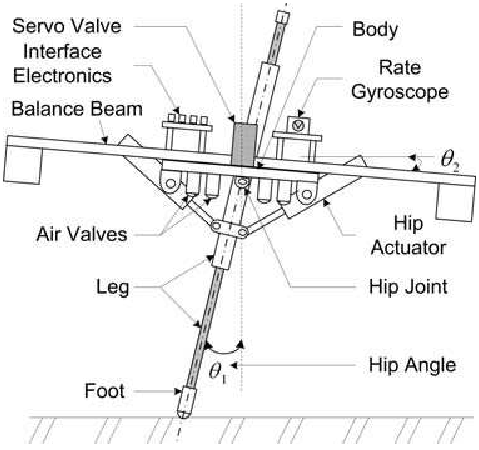
\includegraphics[width=0.4\textwidth]{fig/Rai_2D}}
  \hspace{2cm}
  \subfloat[ARL Monopod I \cite{ARLMono1}] {\label{fig:1_mono1_hip}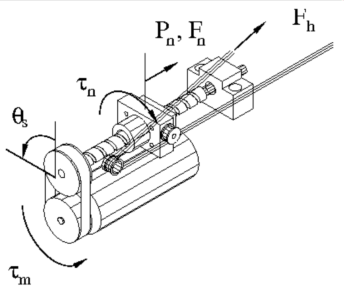
\includegraphics[width=0.450\textwidth]{fig/ARLMono1_hipmotor}}
  \caption[Actively stabilized hoppers]{Actively stabilized hoppers}
  \label{fig:1_activestable}
\end{figure}
\subsubsection{Actively Balanced Robots}
Raibert used a hydraulically actuated hip on top of an articulate leg mechanism for balancing the hopper. The hip actuator used in
the two-dimensional hopper shown in Fig. \ref{fig:1_rai_2D} was pneumatically controlled by varying the pressure gauged by pressure 
sensors on the actuators. The hip can also be moved by means of a winch type actuator as shown in Fig. \ref{fig:1_mono1_hip}. 

\subsubsection{Passive Balancing Robots}
Swinging the leg for active balancing requires energy and people started looking for ways to achieve passive stabilization of
hopper attitude. This kind of stabilization might not provide a complete solution to the problem of stability but certainly reduces
the power consumption of the robot.
After studying ARL Monopod I,  Beuhler incorporated a compliant spring in series with the hip actuator cables as shown in Fig. \ref{fig:1_ARLMono2_sch}. Swinging of the leg could be achieved using the hip-leg spring compliance. Thus a passively stable
running gait was possible for certain initial conditions \cite{Bue_PassRun, ARLMono2}.\\
\begin{figure}[h]
  \centering
  \subfloat[ARL Monopod II \cite{ARLMono2}]{\label{fig:1_ARLMono2_sch}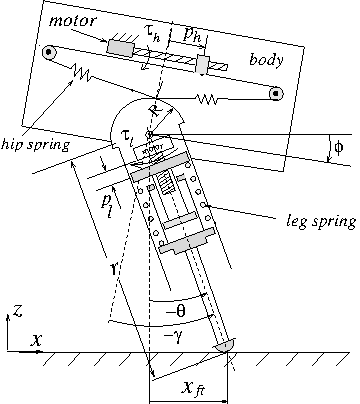
\includegraphics[width=0.4\textwidth]{fig/ARLMono2_sch}}
  \hspace{0.05\textwidth}
  \subfloat[SLOM hopper \cite{sayyad}]{\label{fig:1_SLOM}\includegraphics[width=0.4\textwidth]{fig/SLOM}}
  \caption[Passively dynamically stable hoppers]{Passively dynamically stable hoppers}
\end{figure}

Most of the hoppers reviewed in \cite{review} have their C.G. along the line of action of the impact and spring forces. This provides
a stable system for single place hopping and is referred to as \emph{Springy Leg Inverted Pendulum} (SLIP). It is noted that SLIP
does not account for the pitch stabilization problem which is of practical concern.\\

As shown in Fig. \ref{fig:1_SLOM}, Shanmuganathan et. al. considered asymmetric configurations in which the CG location was offset 
from the geometric center. This is referred to as a \emph{Springy-Legged Offset-Mass} (SLOM) hopper \cite{shanmug}. The robot 
postures at various phases during a hopping cycle are depicted in Fig. \ref{fig:4_rewac}. The impulsive torque acting during the 
stance gives a pitch up velocity in the flight phase. This compensates the net pitch down during the stance phase due to the 
horizontal velocity. Sayyad and Seth have analyzed this configuration using a 3D Poincar\'e map to obtain a periodic motion 
stabilized by observer based state feedback strategy \cite{sayyad}. Fig. \ref{fig:1_wei} shows a miniature 5 cmm tall SLOM hopper developed by
Wei et. al. \cite{5cmhopper}

\vspace{0.4in}
\begin{figure}[h]
\centering
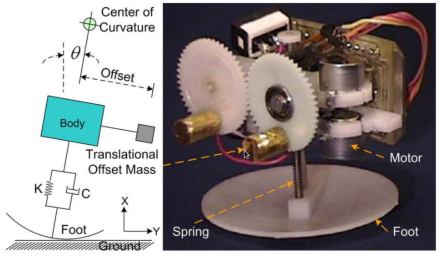
\includegraphics[scale=1]{fig/wei.pdf}
\caption[5 cm tall hopper by Wei]{5 cm tall hopper by Wei et. al. \cite{5cmhopper}}
\label{fig:1_wei}
\end{figure}


















    %\chapter{Problem Statement}
\label{chap:problem}
This chapter discusses previous work on the one legged hopper at IIT Bombay and formulates the exact problem statement and the scope 
for this project.

% 1. sayyad
%     poincar`e map ... read his abstract
%     saboo...sanmukh
% 2. londhe
%     describe mechanism
% 3. simit
%     contributions
% 4. siraj
%     contributions
\section{Previous work}
\subsection{1-D Hopper}
Vitthal Londhe~\cite{londhe} developed a 1D hopper and demonstrated in place hopping capabilities. The design was aimed at minimizing
the energy losses and making the robot easy to assemble and disassemble.
\begin{wrapfigure}{r}{0.4\textwidth}
\centering
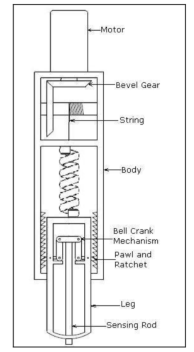
\includegraphics[scale =1.5]{fig/londhe.pdf}
\caption[Vertical Hopper]{Vertical Hopper \cite{londhe}}
\label{fig:2_londhe}
\end{wrapfigure}
Fig.~\ref{fig:2_londhe}, shows the major parts of this hopper viz. a winding motor with the energy pumping mechanism and a telescopic 
leg with a ratchet and paul constraint. The hopper is also confined to a fixed vertical axis. The leg is connected to a compression 
spring. A motor is used to compress this spring.\\

The constraint mechanism consists of a bell crank attached to the paul so that when the leg impacts upon the ground, the paul comes 
free of the ratchet teeth and the spring is free to compress further. This is the first use of impact forces for releasing the energy 
pumping mechanism in a one legged hopper. Thus the motor does not need to do work against the spring force to hold the leg in the compressed position. The latch mechanism mechanically latches the leg in place and unlatches it only when the leg touches the ground.
\subsection{SLOM Hopper}
Fig.~\ref{fig:2_hop2d} shows the prototype developed by Sharma and Gebretsadik~\cite{londhe} for which Vipul Saboo~\cite{saboo} 
designed and fabricated the EPM for it. He could also demonstrate hopping of the robot without active balancing.

The robot consists of a body and a telescopic leg of rectangular cross-section attached to the body by a spring. The leg also has a 
freely rotating ankle with a foot attached to it. The ankle ensures that the foot always falls flat on the ground irrespective of the 
orientation of the robot while touchdown.\\
\begin{figure}
\centering
\subfloat[SLOM hopper : sketch]{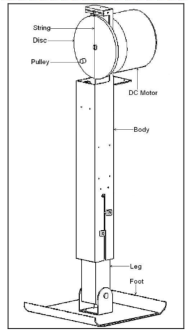
\includegraphics[scale = 1.5]{fig/saboo.pdf}\label{fig:2_hop2d}}
\hspace{1in}
\subfloat[Paul and ratchet]{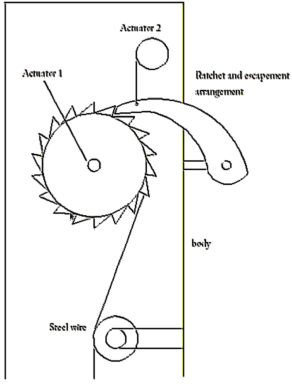
\includegraphics[scale = 1.2]{fig/ratchet.pdf}\label{fig:2_ratchet}}
\caption[2D SLOM hopper]{2D SLOM hopper \cite{saboo}}
\label{fig:2_saboo}
\end{figure}
To reduce the friction between the telescopic leg and the body, teflon bearings are used in sets of two on each of the four sides of 
the leg. The construction of the robot makes it very difficult to assemble and disassemble it. Also, the mass of the leg is almost 
${2/3}^{rd}$ of the mass of the body which results in huge energy loss of the system during impacts.
The EPM consists of a ratchet and a pawl with a voice-coil which activates the pawl. The voice-coil is electrically actuated by a 
mechanical limit switch attached on the foot of the robot. There is also a latch-type EPM where the motor can be switched off after 
the spring is compressed.\\

Simit \cite{simit} developed a treadmill and constraining mechanism (TCM) for the SLOM hopper. He also demonstrated an embedded system
for hopping height control using a feed-forward and PID controller. A ground station for gathering telemetry data from the TCM 
interface.

\subsection{Reaction wheel}
Siraj \cite{siraj} modeled attitude control of the hopper as a position control problem for the reaction wheel pendulum. He
demonstrated PID and LQR control strategies for the reaction wheel pendulum. Optimal control strategies have to be looked into because
as observed by Beuhler \cite{Bue_PassRun, ARLMono2}, almost 50\% of the total energy is utilized in swinging the leg mass i.e. in
attitude reorientation. A inertial measurement unit (IMU) using a complementary filter was also developed.

\section{Problem formulation}
The SLOM hopper was used as a test bed for devising hopping strategies by Saboo \cite{saboo}, Simit \cite{simit} and Siraj \cite{siraj}. However, it was an over-designed system with large energy losses due to impacts and friction. It was necessary to
remove these flaws in the robot before further work could be done on it. Hence, it was decided to go ahead with a completely new
mechanical design for the hopper keeping the following things in mind about the previous design.
\begin{enumerate}
\item
SLOM concept is quite novel and the new design will be based on it.
\item
Compression spring need an enclosure outside them to keep them in place when in compression. This results in frictional losses in
every cycle of energy pumping. Tension springs on the other hand do not have such frictional losses associated with them. It was thus
decided to use tension springs for the new design.
\item
The SLOM hopper could not hop above a height of 10 cm. The energy pumping mechanism (EPM) was the limiting factor. For achieving heights larger than this, we need to significantly reduce the leg mass and have a more energy efficient EPM.
\item
A reaction wheel should be present on the hopper and this will be used to reorient the robot to demonstrate both in-place hopping
and running capabilities.
\item
An embedded system along with on-board power supply shall be used to control the actuation, sensors and execute the control law.
\end{enumerate}



    \chapter{Mechanical Design}
\label{chap:mech_design}
As pointed out in the previous chapter, the major task of this project was to devise an efficient mechanical
design. Two different designs both based on extension springs were looked into. 
This chapter describes them and the motivation behind choosing the final design to be fabricated.

\section{Design 1}
%Write general description of design 1 here.
\subsection{Energy pumping}
\begin{figure}[!h]
\centering
%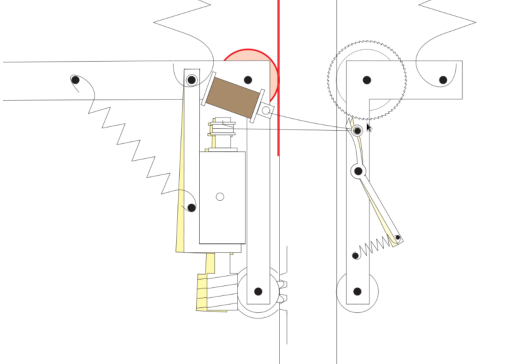
\includegraphics[scale=0.5]{fig/seth_design.pdf}
\caption{Winding motor with pulley on the leg}
\label{fig:3_pratik_design}
\end{figure}
Fig. \ref{fig:3_pratik_design} shows the pulley mechanism for storing energy in the large central spring.
The winding motor is placed upon the platform which can be called as the larger mass M of the two mass
system. A winch connects the motor to the same platform passing over the pulley on the lower leg. Thus, as
the motor rotates, it pulls the platform (and itself) downwards while extending the spring above it. 
A few points to note about the energy pumping design are,
\begin{enumerate}
\item
The motor has to move a distance twice that of the extension of the spring. This is
especially important when we look at the timescales over which we have to extend the spring, these are around
200-300 msecs. A larger distance in smaller time results in a large $\omega$ for the motor which translates
to a smaller available torque. This neccesitates a larger motor that can provide this torque. 
\item
The large mass of the platform (M) is helping in the extension of the spring and hence the torque required
for the winding motor reduces.
\item
It has to be ensured that the winding winch does not slip over the pulley when the platform is suddenly released from
the constraint. At the same time, the winch must be free enough so as not to hinder the movement of the platform after
the release.
\end{enumerate}

\subsection{Constraint}
\begin{figure}[!h]
\centering
%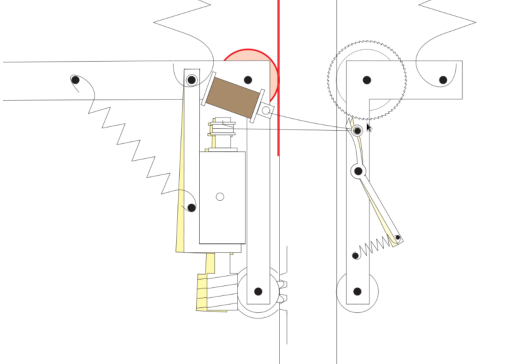
\includegraphics[scale=0.5]{fig/seth_design.pdf}
\caption{Constraint for the pulley}
\label{fig:3_pratik_constraint}
\end{figure}
Fig. \ref{fig:3_pratik_constraint} shows the constraint mechanism for the pulley. It consists of a hatch connected to
the lower leg with a torsional spring. The toothed part of the pulley is free to move in the clockwise direction (thus
compressing the torsional spring every time). The lower part of the leg is cylindrical with a top flange which matches
the top face of the cylindrical bushing shown inside the main leg. Thus the lower leg can move only up. The protruding
portion of the main leg prevents the hatch from moving in the clockwise direction, thus constraining the pulley from
rolling back in the anti-clockwise direction.
\begin{itemize}
\item
The diameter of the lower leg is expected to be around 2-3 cms and it is difficult to fabricate the hatch on such
a small surface.
\end{itemize}

\subsection{Using the impact for energy release}
This design is unique because it utilizes the impact force ($m\:v_{touch-down}$) to release the stored energy in the main
spring. Visualize the lower leg impacting on the ground. This results in the hatch (which is holding the pulley from
moving back) impacting against the protrusion of the main leg. Since the impact force is easily larger than the torsional
spring force, the hatch closes and the lower leg goes inside the main leg thus enabling free rotation of the pulley. There
is a compression spring inside the main leg connected to the lower leg which gets compressed while this happens. It is
responsible for pushing the lower leg back outside after $t_{liftoff}$.

\section{Design 2}
\begin{figure}[!h]
\centering
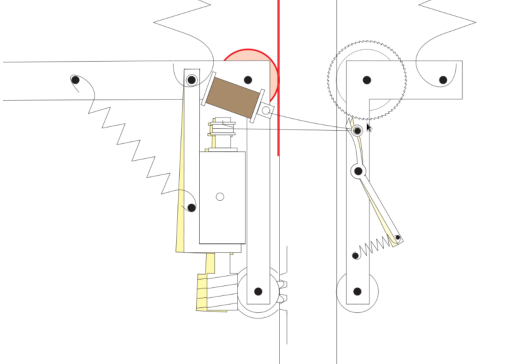
\includegraphics[scale=1.8]{fig/seth_design.pdf}
\caption{Rack and pinion on the leg with the drive motor}
\label{fig:3_seth_design}
\end{figure}

\subsection{Energy pumping}
The leg consists of a rack on one of its sides. A single dual shaft motor in a sleeve is used to drive the pinion
on this rack as
well as pull the paul to free the ratchet. This motor consists of a string attached to a friction pulley on the shaft.
A friction pulley is a device whose coupling is dependent upon the speed of the relative motion between the two surfaces.
Thus, the motor can pull the paul only beyond a certain $\omega$. Below this speed, the paul spring is strong enough to
engage it with the ratchet. After the paul engages, the string becomes slack again.

\subsection{Constraint} 
The platform and the ratchet are rigidly connected to a band drive which rolls along
the length of the leg. This ensures that contact of the roller inside the band drive and the leg is maintained at all
times. Since the ratchet is rigidly connected to the platform, both can only move together i.e. only when the paul is
pulled by the drive motor. 

\subsection{Energy release}
This design uses an electromechanical system to release energy. After sensing the impact through a touch switch located
below the leg, we can use a voice coil actuator to pull the string which in turn moves the paul. This brings in the pull
back spring attached to the sleeve into the picture and it prompty pulls the sleeve away from the rack. Note that the string attached 
to the drive motor pulley is slack at this point.

\subsection{Evaluation}
\begin{itemize}
\item
The worm-worm wheel on the rack mechanism provides a huge mechanical advantage and thus reduces the maximum torque required from
the motor. This scales down the mechanical system as well as the electronic system requirements.
\item
The friction pulley has to work against the pual spring, sleeve spring and the horizontal component of the rack force ($k\:x\:tan\:\theta$) to keep the string in tension. This is compounded by the fact that the there is a maximum $\omega$ the motor can
accelerate to in the energy storing phase. It is much better if this $\omega$ is dictated by the torque requirements which are as
critical rather than this mechanism.
% \item
% Voice coil actuators take up a lot of energy and can be replaced by a servo motor instead. The torque calculations for this are yet
% to be done.
\end{itemize}






    \chapter{Sizing of Hardware}
\label{chap:sizing}
We looked at two designs in Chapter \ref{chap:mech_design}. This chapter describes some simulations done
for the sizing of various components. The major parts of this process are,
\begin{enumerate}
\item
Masses of the platform and the leg
\item
Dimensions of the reaction wheel based on the above masses
\item
Choice of winding and reaction wheel motors
\end{enumerate}

\section{$2$ mass problem}
\begin{figure}[!h]
\centering
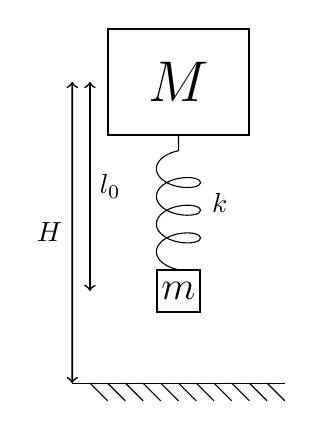
\begin{tikzpicture}[scale=0.45]
\draw (-3,0) -- (3,0);
\foreach \x in {-2.5,-2,...,2.5}
\draw (\x,0) -- (\x+0.5,-0.5);

\path (-2,7) coordinate(M1);
\path (2,10) coordinate(M2);
\path (-0.6,2) coordinate(m1);
\path (0.6,3.2) coordinate(m2);

\draw [thick](M1) rectangle (M2) node[midway]{\huge{$M$}};
\draw [thick](m1) rectangle (m2) node[midway]{\Large{$m$}};

\path (-2.5,0) coordinate (O);
\path (-2.5,2.6) coordinate (SPL);
\path (-2.5,8.5) coordinate (H);

\draw[<->] [semithick](O)++(-0.5,0) -- (-3,8.5) node[midway, left]{$H$};
\draw[<->] [semithick](SPL) -- (H) node[midway, right]{$l_0$};


\draw[snake=coil, segment amplitude=8pt] (0,3.2) -- (0,7) node[midway,right=2ex]{$k$};
\end{tikzpicture}
\caption[2 mass problem]{2 mass problem \cite{simit}}
\label{fig:4_2mass}
\end{figure}
The basic idea behind a hopper is like that of the 2 masses connected by a spring problem. If the system shown in Fig.
\ref{fig:4_2mass} is allowed to fall from a height, the heavier mass pulls the smaller mass with it back into the air
after impact. Every cycle is accompanied by a loss in energy due to the inelastic impact of the smaller mass with the
ground. If we pump this energy back into the system using an external agent in every cycle, we can ensure sustained
hopping at the chosen height. The 2 mass problem can thus be taken as a basis to compute the range of values of masses
for acceptable performance. The following assumptions have been used in the simulation that follows,
\begin{enumerate}
\item
Dropping height (H) : 0.6 m
\item
Spring constant (k) : 300 N/m
\item
Spring relaxed length ($l_0$) : 0.3 m
\item
Trapezoidal profile for $\omega$ of the winding motor (constant $\alpha$ at the start and end)
\item
Design 1 was used as the base for this simulation. It is expected that the total torque requirements will
reduce due to the mechanical advantage provided by the rack and pinion design as shown in Fig. \ref{fig:3_seth_design}.
\item
Neglect energy loss due to friction
\end{enumerate}
It is seen from Fig. \ref{fig:4_2mass} that if $h_i$ are progressive heights, we have the relation,
\begin{equation}
h_n = \frac{Mh_{n-1} + ml_0}{M + m}
\end{equation}
\begin{equation}
\label{eqn:4_eloss}
E_{loss} = \frac{Mg\;(H-l_0)}{1 + M/m}
\end{equation}

\begin{figure}[!h]
\centering
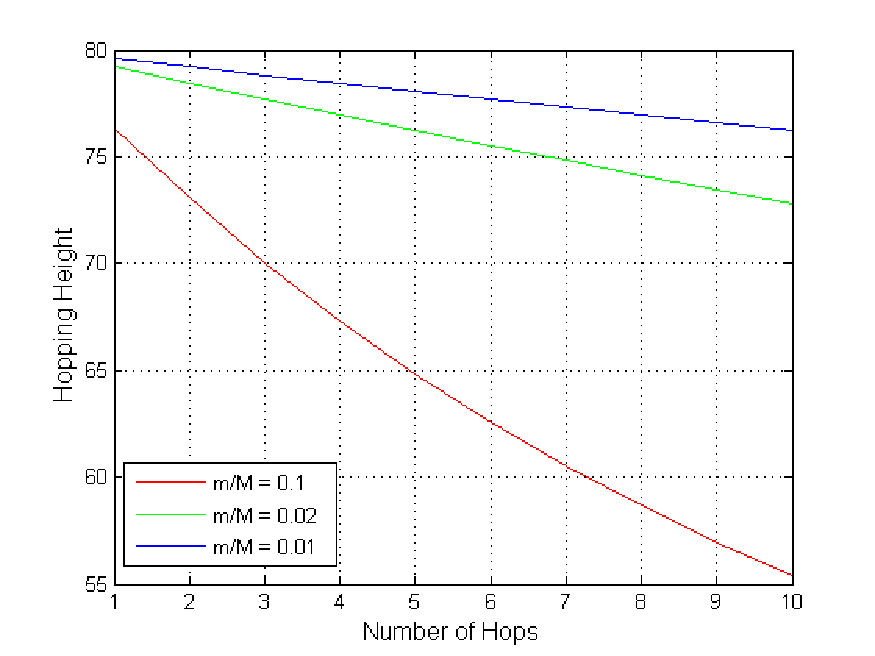
\includegraphics[scale=0.8]{fig/2mass_hopheight.pdf}
\caption{Hopping height for different M/m}
\label{fig:4_hopping_height}
\end{figure}
From Fig. \ref{fig:4_hopping_height}, it is seen that larger the ratio M/m, i.e. smaller the leg
mass, less is the loss in energy resulting in more number of hops. This is also seen for a increasing M. We would however,
like the M to be within limit too as we will also need to pump in extra energy into the system if the desired hopping
height is more than the starting height.\\
\begin{figure}[!h]
\centering
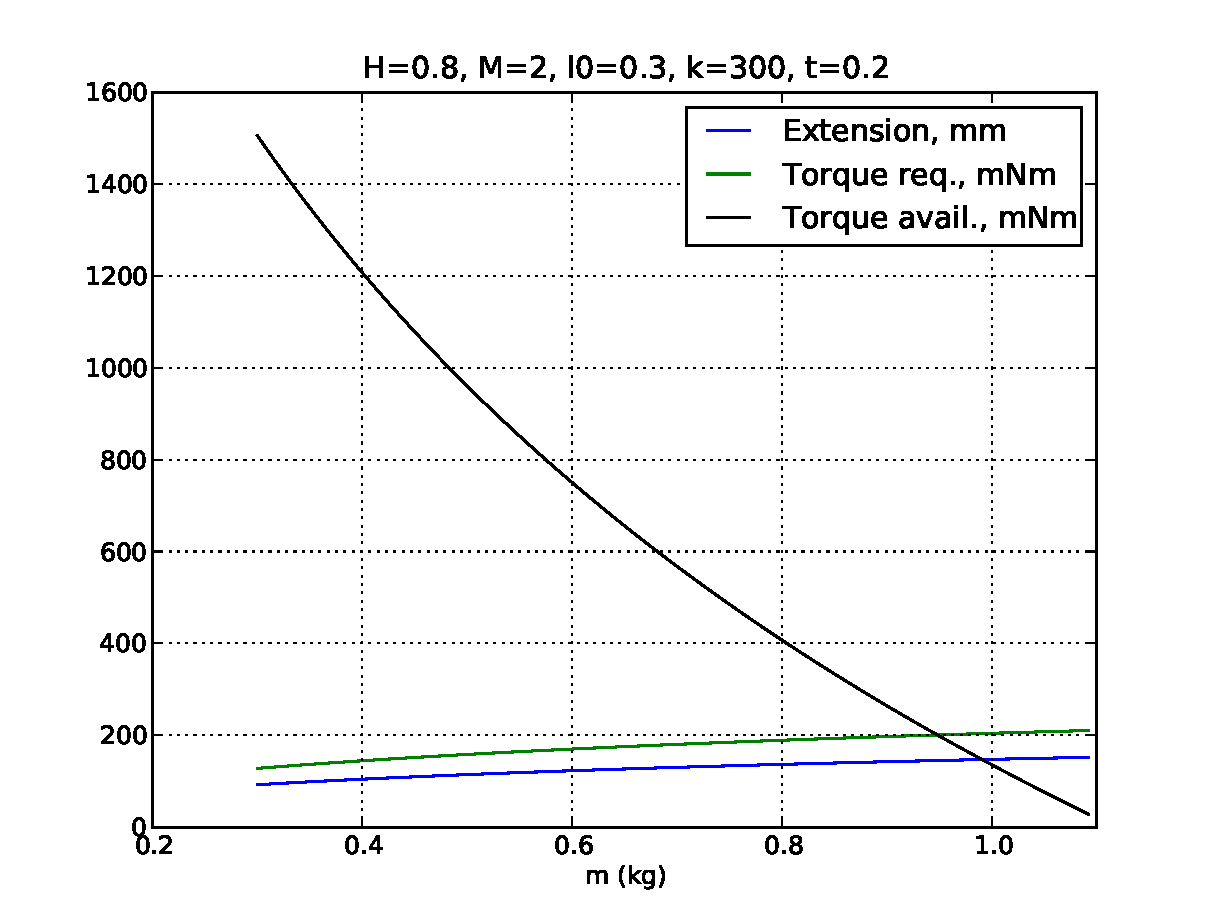
\includegraphics[scale=1.5]{fig/2mass_m.pdf}
\caption{Torque variation with m}
\label{fig:4_torque2mass}
\end{figure}

Fig. \ref{fig:4_torque2mass} shows the required torque  for extending springs to compensate the energy lost during impact fully within 0.2 sec. This simulation has been plotted for Design 1 from Chapter \ref {chap:mech_design} with a pulley radius of 2 cms. It is
observed that m is the single most important parameter in hopper design. The required torque is a very strong function of the leg mass. As this mass increases, we need a larger motor to satisfy torque requirements. It is noted that a value of about 0.4--0.6 kg
can be called a reasonable estimate for the leg mass as we can easily choose a motor delivering the required torque for these values.\\

It is also seen that an extension of about 11 cms with a single spring of k = 300 Nm is needed to compensate the energy loss for 
hopping heights of 80 cms. So we should ensure that we can provide a maximum extension around 15 cms.

\section{Impact analysis}
\label{sec:4_impact}
The desired hopping height dictates a hopping frequency. Intuitively, smaller hopping height results in large number of impacts per time
and consequently in larger energy loss per unit time. This is seen from Fig. \ref{fig:4_freq_height} because the hopping frequency is closer to the natural frequency for small hopping heights. However, beyond this consideration, since the hopper is a spring mass
system, it possesses a natural frequency of its own. If the hopping frequency is near to this natural frequency, a large
amount of energy is taken away by impact forces in every cycle. We intend to arrive at a range of values for the masses
to ensure a large difference between the hopping frequency ($\omega_{hop}$) and the natural frequency ($\omega_{nat}$).
The details of this analysis are as follows,
\begin{itemize}
\item 
Conserve energy at H and the moment of maximum extension of the spring after $t_{touchdown}$ to get the minimum height of the
fully extended platform above the leg. This comes out to be 8 cms for m = 0.4 kg. This value also reduces with increasing m. I
assumed no pre-extension of the spring while calculating this. The final value will be less then 8 cms if we take it into account.
Thus we say that the leg should protrude about 12 cms beyond the maximum extension of the platform which is obtained from Fig.
\ref{fig:4_hopping_height}.
\item
If $x_2$ is the height of C.G. just before touchdown, we can calculate the time taken for it to fall from a height H to $x_2$ as
$t_1$.
\item
M undergoes simple harmonic motion from time $t_1$ till liftoff, and this time of motion is $t_2$
\item
M transfers its momentum at $t_1 + t_2$ to m resulting in a velocity $v_{cg, t_{2}}$ for the C.G. To ensure that M has largest
velocity while transferring momentum to m, we need to put a mechanical stopper at the natural length of the spring.
\item
The resultant velocity is just enough for the C.G. to reach a height H in time $t_3$.
\item
Total hopping time T = $t_1 + t_2 + t_3$, with $\omega_{hop} = \frac{2\pi}{T}$.
\item
$\omega_{nat} = \sqrt{\frac{k\;(1+m/M)}{m}}$
\end{itemize}

\begin{figure}[!h]
\centering
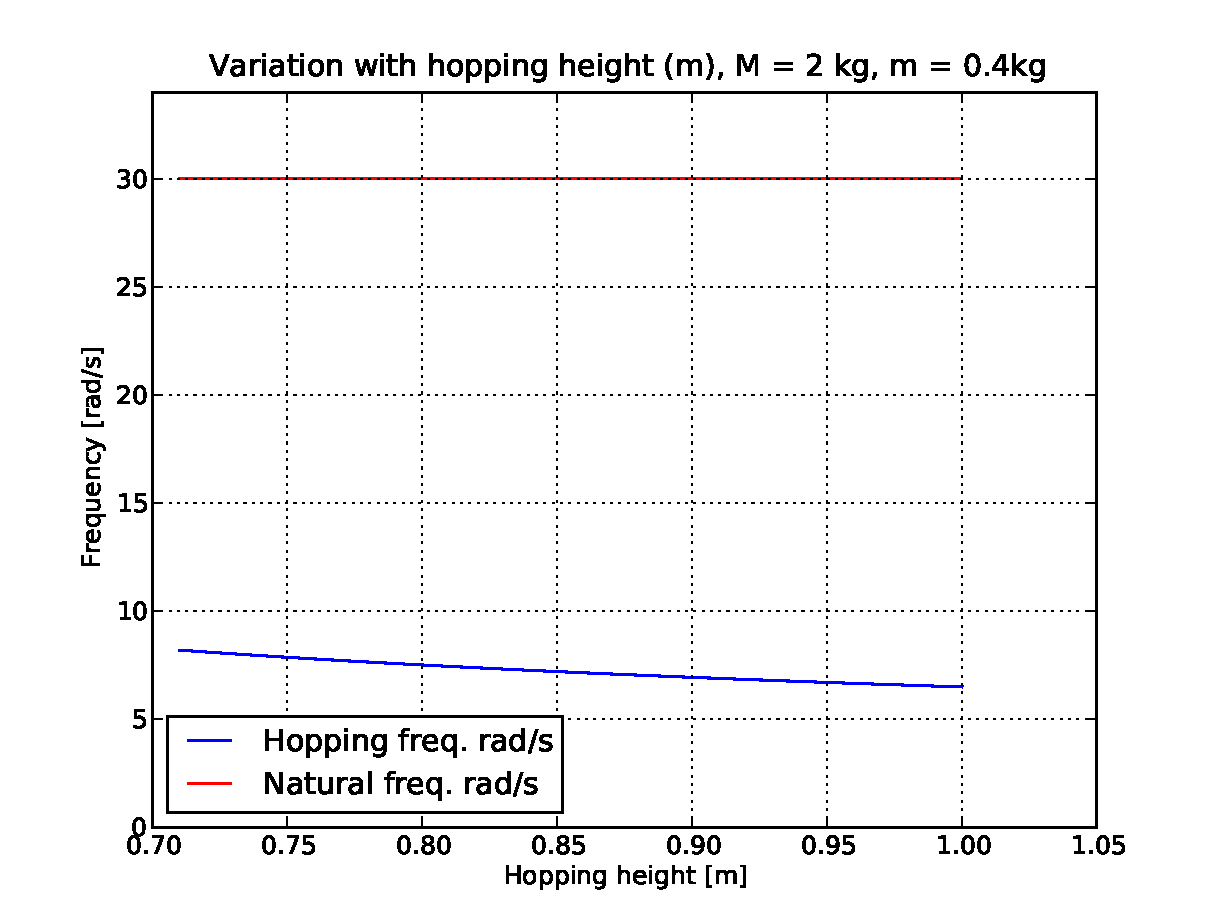
\includegraphics[scale=1.8]{fig/freq_hopheight.pdf}
\caption{Frequency variation with hopping height for M/m = 5}
\label{fig:4_freq_height}
\end{figure}
Fig. \ref{fig:4_freq_height} shows that $\omega_{hop}$ and $\omega_{nat}$ are separated by large gap for the usable range
of values of hopping height. A similar analysis for variation of M also reveals that the two frequencies are separated
by a large gap for all usual values.
\begin{figure}[!h]
\centering
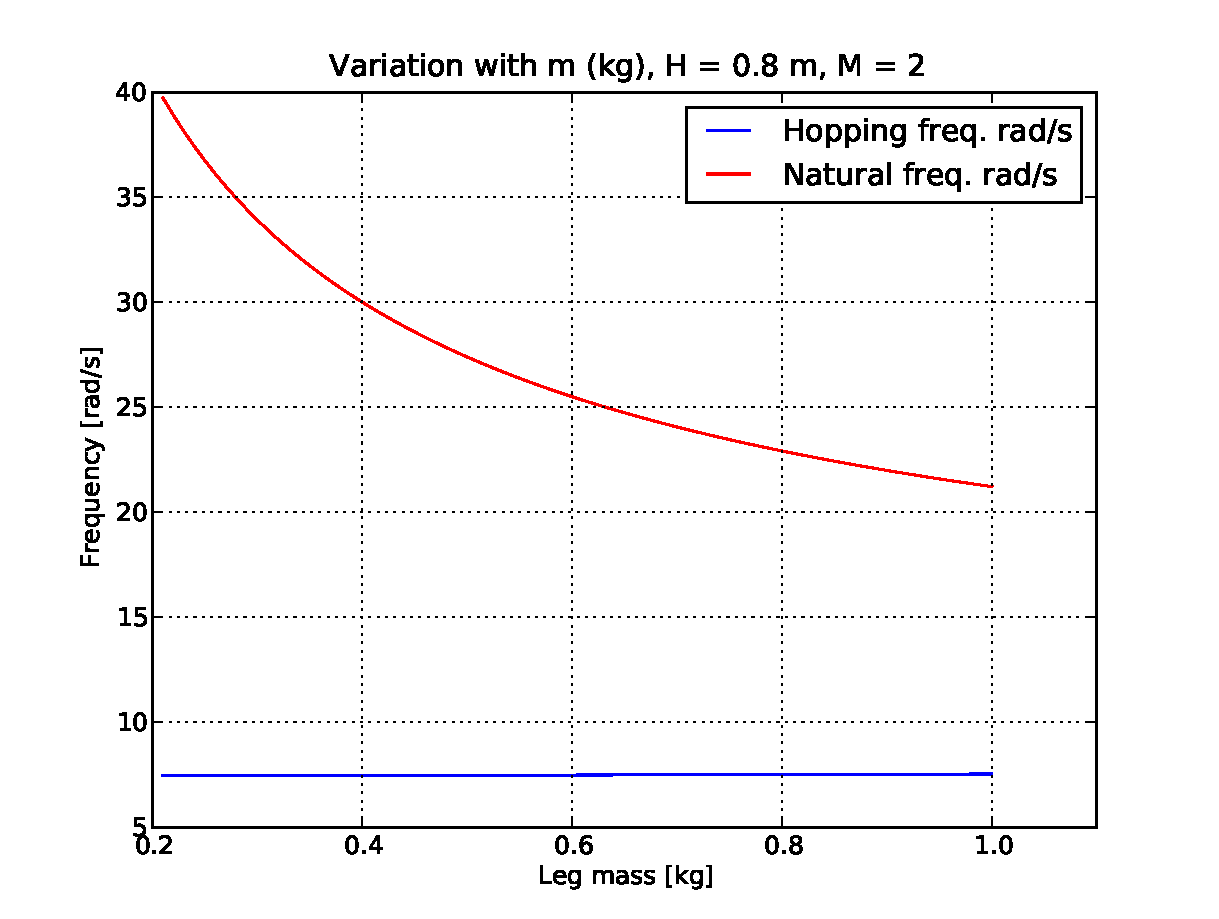
\includegraphics[scale=1.5]{fig/freq_m.pdf}
\caption{Frequency variation with m}
\label{fig:4_freq_m}
\end{figure}
Fig. \ref{fig:4_freq_m} succinctly depicts all the above analysis. As the leg mass increases, the hopping frequency goes
closer to the natural frequency i.e. more impact per unit time. To compound matters, more and more energy is lost per impact
as per Eqn. \ref{eqn:4_eloss}. So the conclusion from impact analysis is that the leg mass should be as low as possible. It is also
seen from Fig. \ref{fig:4_freq_m} that \mbox{m = 0.4 -- 0.6 kg} is a good solution as well as an achievable one. 

\section{Reaction wheel}
\label{sec:4_rewac}
For achieving a running gait with the hopper, it has to be started with the exact initial pitch and horizontal velocity.
For any other initial condition, the hopper is pitch unstable and will not be able to continue the running gait.
As mentioned in \cite{shanmug}, an offset mass acts as a passive stabilization to the pitch attitude of the hopper.
To get rid of this need for exact initial condition which is quite impractical, we design a reaction wheel on the hopper.
This will result in torque coupling on the pitch axis and thus provide an active control over the pitch of the robot.
The coupling equation can be written as,
\begin{equation}
J_{wheel}\;\omega_{wheel} = -(J_{wheel} + J_{body})\;\omega_{body}
\end{equation}
\begin{figure}[!h]
\centering
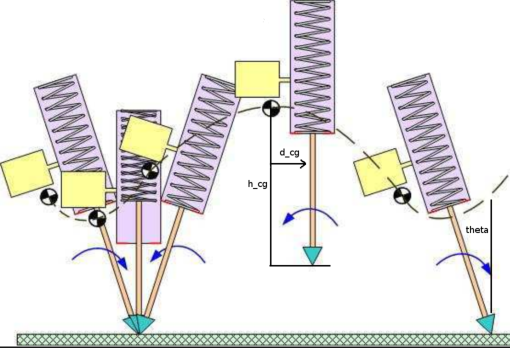
\includegraphics[scale=1]{fig/slom_motion.pdf}
\caption{Stabilizing impact torque due to SLOM}
\label{fig:4_rewac}
\end{figure}
Let us look at the various stages of reaction wheel stabilization,
\begin{itemize}
\item
Let $\theta_{impact}$ be the impact pitch attitude and $\theta_{liftoff}$ be the lift-off attitude. Pitch is measured with respect to
the vertical direction. An upright hopper means a pitch of zero.
\item
From Fig. \ref{fig:4_rewac}, the stabilizing impact torque is given by \mbox{$\tau = m\:v_{impact}\:(h_{cg} sin\:\theta + d_{cg} cos\:\theta)$}. This is a positive torque and generates a pitch up. Also, \mbox{$\omega_{liftoff} = \tau_{impact}\:/J_{body}$}
\item
The angle rotated due to horizontal velocity in the stance phase is $\Delta\:\theta = -v_h\:/h_{cg}\:\Delta\:t$ where $v_h$ is the horizontal velocity. This means
$\theta_{liftoff} = \theta_{impact} + \Delta\:\theta$.
\item
The lift-off pitch needs to be corrected to $\theta_{impact}$ while the hopper is in the air. $\omega_{liftoff}$ might not be enough
to correct this pitch and so we need an additional reaction wheel.
\end{itemize}
The following assumptions were made during the analysis for the reaction wheel,
\begin{itemize}
\item
The reaction wheel is taken as a ring with mass of 1.5 kg concentrated at the rim.
\item 
It is easy to see that for any given horizontal velocity, there exists a particular impact pitch which results in stable gait without a reaction wheel. Our objective is thus to go to this impact pitch angle from any
given initial condition such as a zero pitch angle.
\item
We consider the case where the pitch is such that we have no horizontal velocity and no stabilization impulse from the ground. This pitch is reoriented to 30 degrees within one hop which corresponds to a huge horizontal velocity of 13.5 m/s. The stable pitch will be less than this for lower velocities. In actual operation
there will be large reaction wheel torques only while converting the initial condition into a stable
running gait. After that there will only be small control torques about the stable pitch angle.
\item
We assume a trapezoidal profile for $\omega_{wheel}$ with length of the plateau taken as $T_{air}/2$. The acceleration phase is
$T_{air}/5$ on either side. This means that we finish the reorientation task within 9/10 ths of the time that the hopper remains in the air in the first hop ($T_{air} = t_1 + t_3$ from Section \ref{sec:4_impact}).
\end{itemize}


\begin{figure}[!h]
\centering
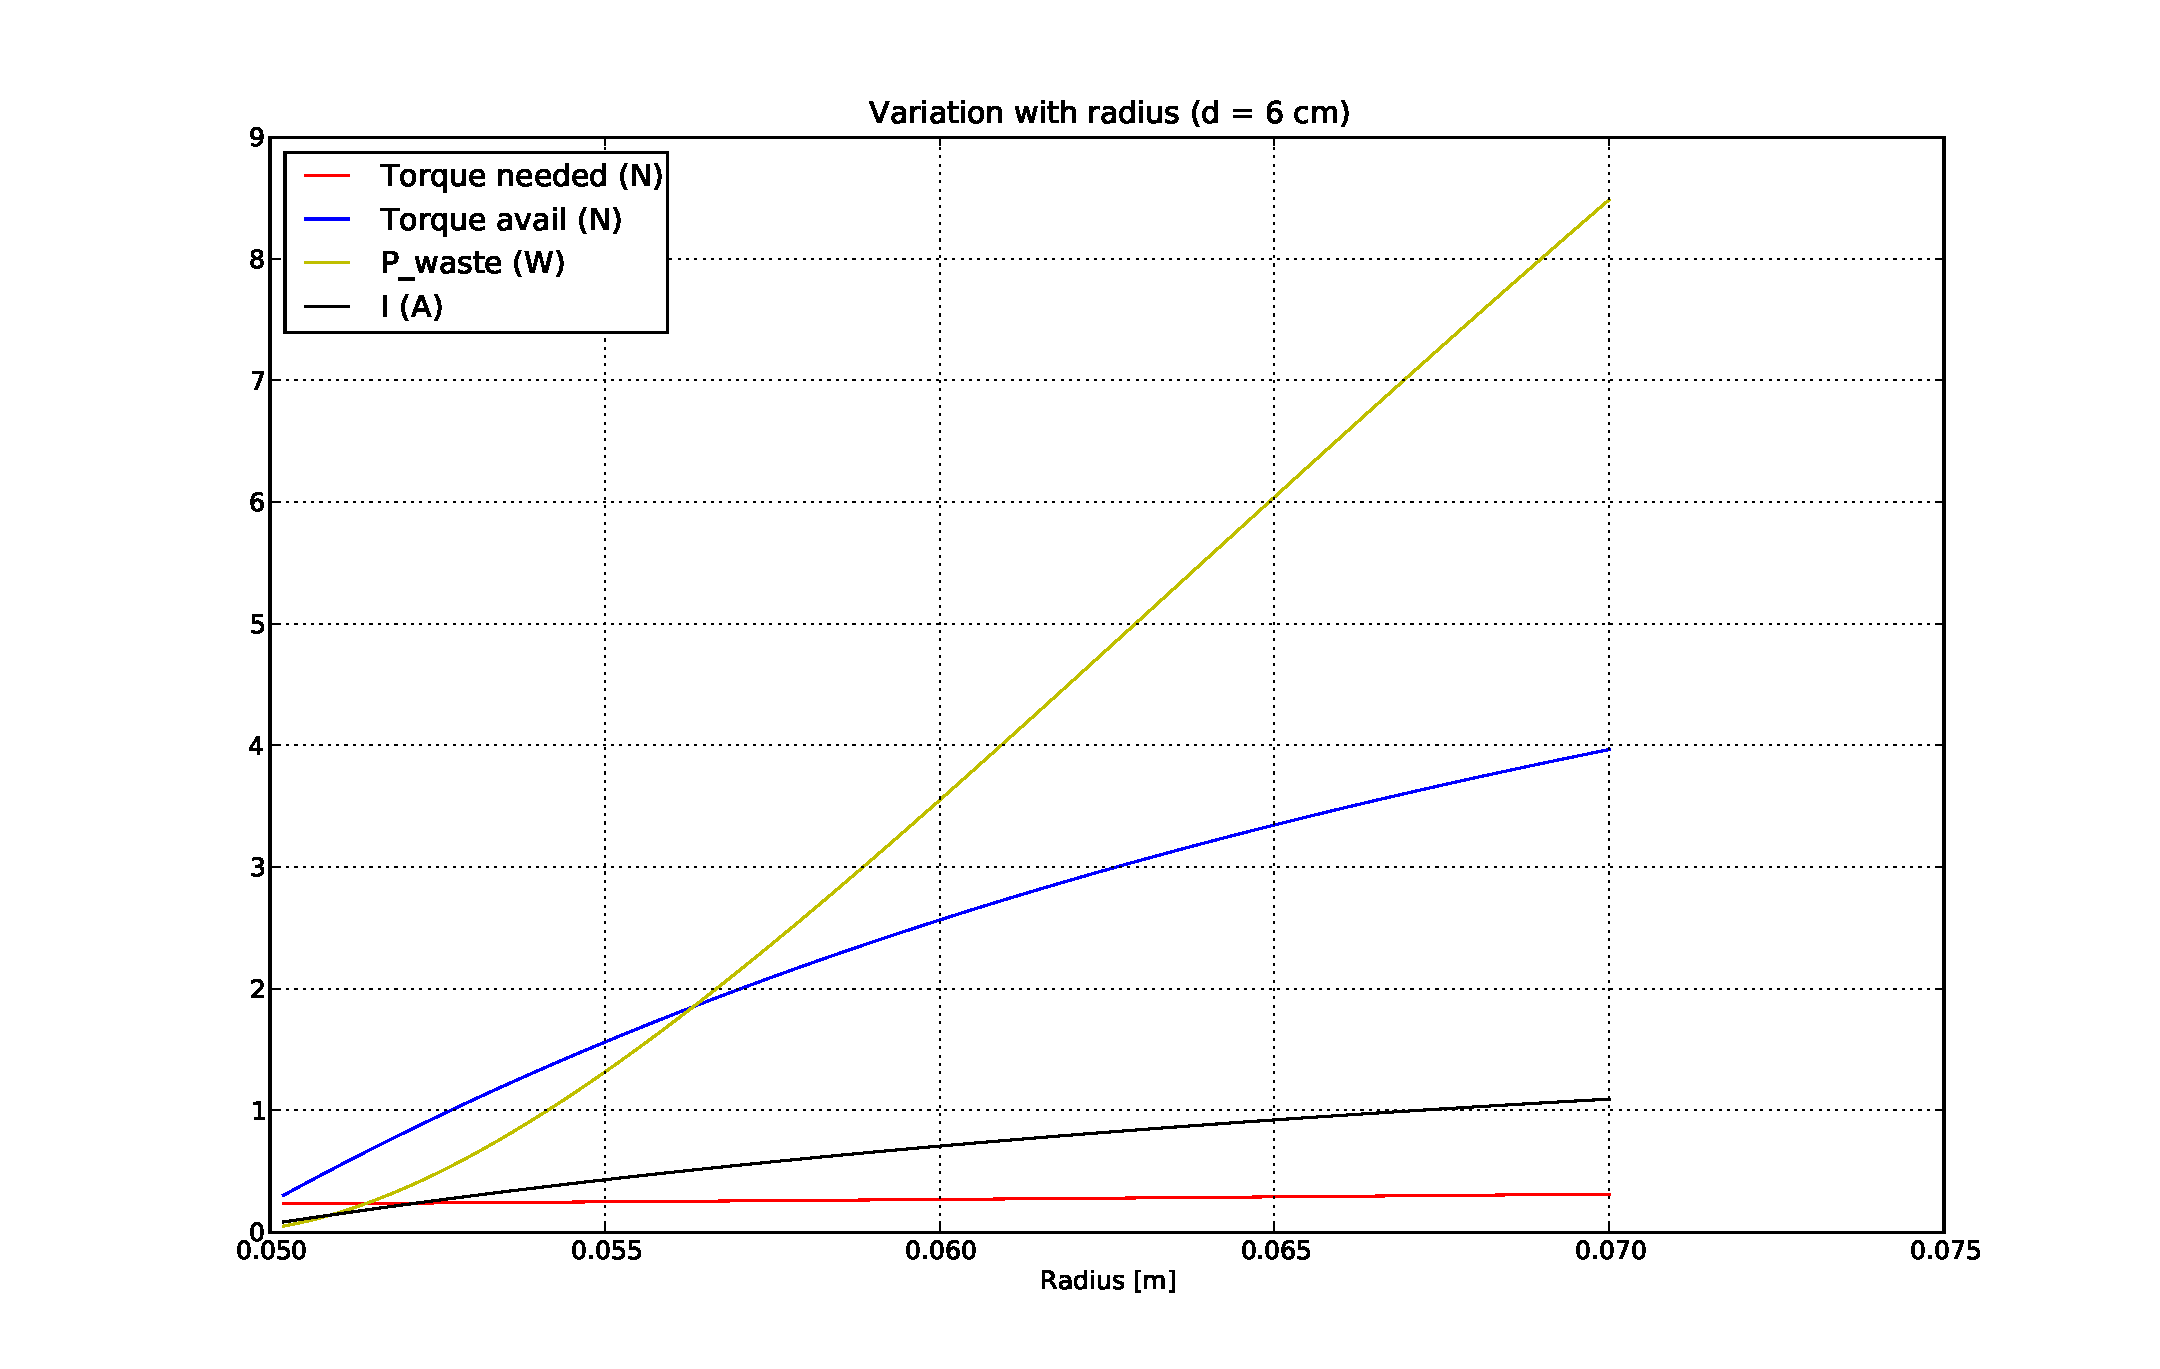
\includegraphics[scale=1.4]{fig/rewac_radius.pdf}
\caption{Torque requirements vs wheel radius}
\label{fig:4_rewac_radius}
\end{figure}
\begin{figure}[!h]
\centering
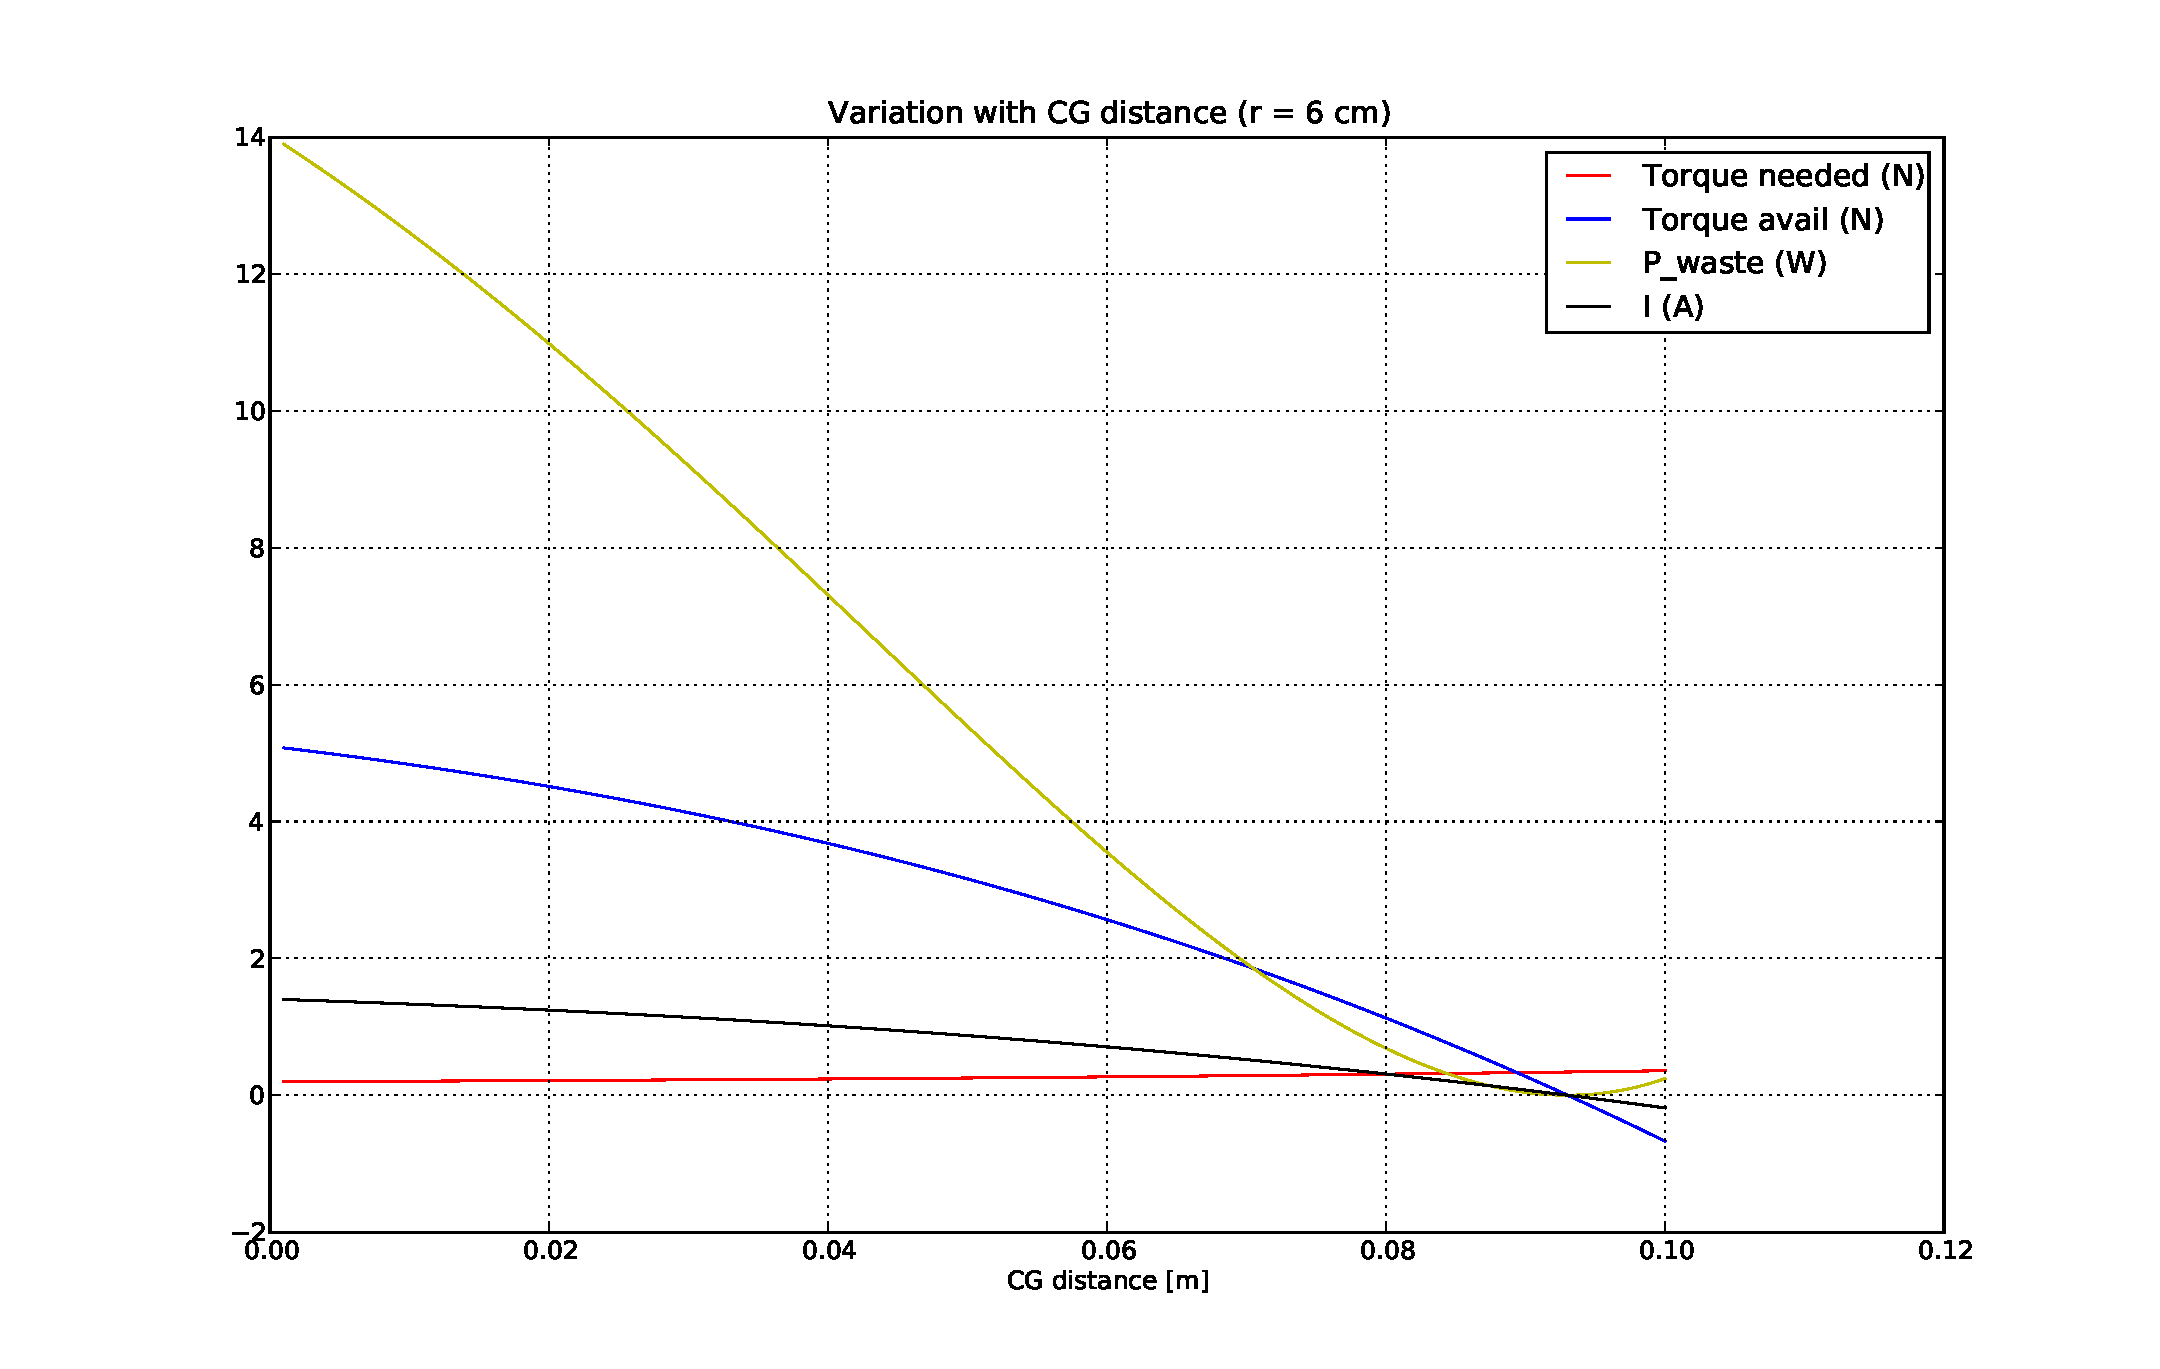
\includegraphics[scale=1.4]{fig/rewac_dist.pdf}
\caption{Torque requirements vs C.G. offset}
\label{fig:4_rewac_dist}
\end{figure}

\subsection*{Results}
Figs. \ref{fig:4_rewac_radius} and \ref{fig:4_rewac_dist} have been plotted for distance of C.G. = 6 cms and
radius of the reaction wheel taken as 6 cm (mass = 1.5 kg). We can see that the required torque for reorientation as mentioned in above is around 500 mNm with output power being around 1.5 W.

\section{Choosing Components}
\subsection*{Reaction wheel motor}
Figs. \ref{fig:4_rewac_dist} and \ref{fig:4_rewac_radius}, were plotted for a 2342CR024 motor. We bump up
the gear ratio to achieve a higher available torque as compared to the necessary torque. There is a trade off
here because we also want a particular value of $\omega$ for reorientation. We thus choose to suffer on the
amount of wasted power to achieve these dual objectives. The gear-box thus chosen is one with a standard 139 : 1 ratio. The motor was chosen by looking at the currents required for different motors. The current required
for this motor is around 1.2 A.

\subsection*{Drive motor}
We look at Fig. \ref{fig:4_torque2mass} to choose the drive motor. For the purposes of design, we take common values of worm-worm wheel diamter ratio (0.5), pressure angle (20 deg), helix angle for worm (25 deg) and co-efficient
of friction $\mu = 0.3$. The torque required from the motor is not more than 200 mNm. The total power required
for this task is about 4.5 W. We choose the same 2342CR024 motor for this task. The gear box is taken as a
43 : 1
standard one to ensure that we are operating at the rated motor speed. This results in less energy wastage. There need not be any optical encoders for this motor as we will be measuring the velocity of the extension using encoders at the band drive. The currents for this operation are always below 1.5 A. Hence we can use a relatively small motor driver like Texas Instruments DRV 8801 to drive this motor.



    \chapter{Attitude Estimation}
\label{chap:kf}

\section{Introduction}
\begin{figure}[!h]
\centering
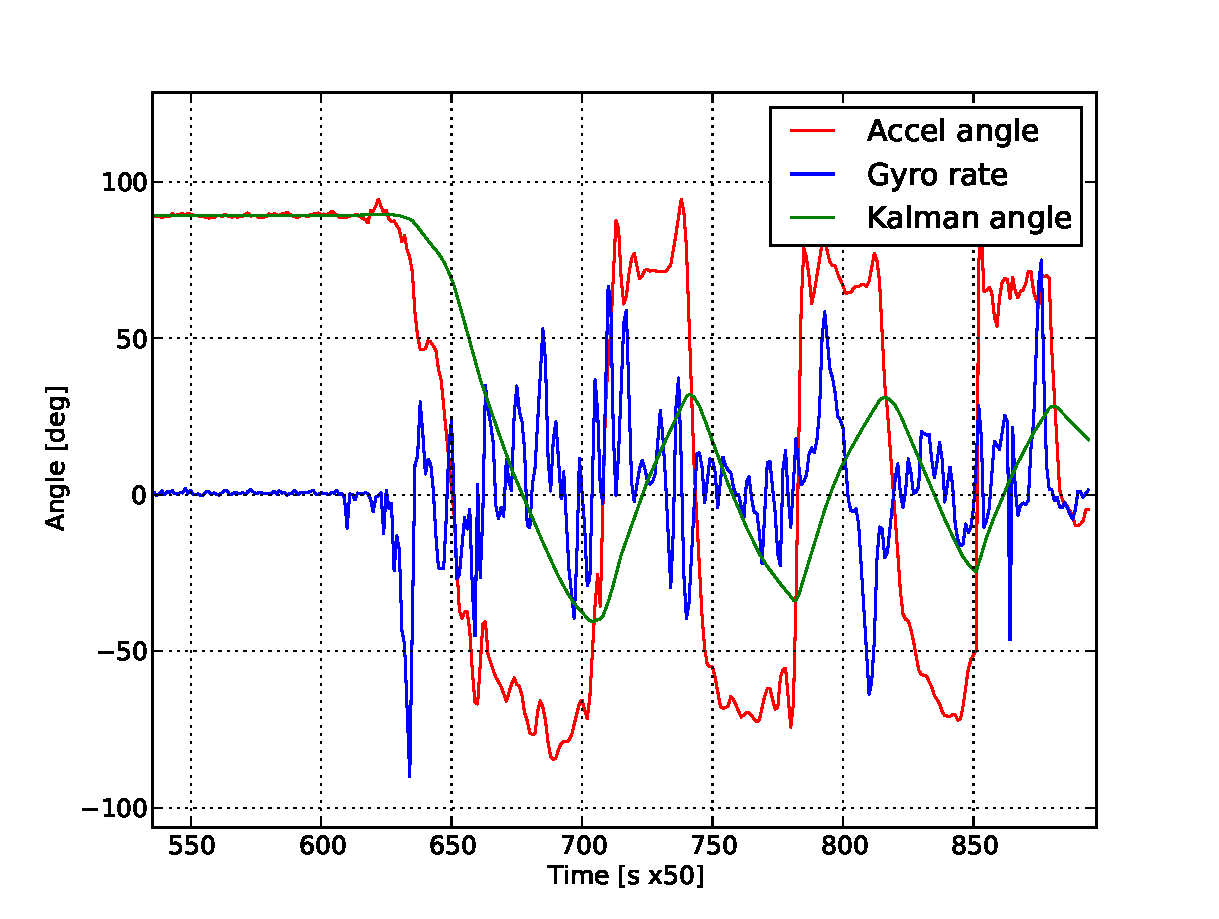
\includegraphics[scale=0.8]{fig/kalman_lowfreq.pdf}
\caption{Kalman filter : Low frequency input}
\label{fig:5_kalman_lowfreq}
\end{figure}
As shown in Fig. \ref{fig:5_kalman_lowfreq}, the readings of the gyroscope and the accelerometer
are highly noisy and erratic even in the situation of smooth movements of the IMU. This shows,
that depending upon either of the two sensors is not good for pitch estimation. Gyroscopes are
high frequency sensors and accurately estimate the rate. However, they also show pronounced
variation of readings with time (gyro bias) and temperature (compensated to an extent). 
Accelerometers are good at low frequency measurements. These do not suffer from a growing
bias like the gyroscopes and can be used to correct the readings estimated on the basis of
gyroscope rate from time to time. We look at Kalman filter as a way to fuse these two sensors.\\

Various alternatives for filtering schemes exist and complementary filters are very widely used
for fusing accelerometers and gyroscopes on IMUs. I decided to use a Kalman filter because
the micro-controller can easily handle the computations at usable update rates of about
20-50 Hz. This is one of the major reasons cited in literature for the use of complementary
filters over Kalman filters. It is also noted that for linear systems, there is little difference in the equations of the two filters.\\

\section{Equations}
The equations for Kalman filter with a state vector $\bm{x} = [x_1\;\;x_2]^T = [\theta\;\;\dot{\theta}]^T$ are give below.\\

State equation :
\begin{equation}
\label{eqn:5_kalmanstate}
\bm{x}_{k+1} = \bm{A}\:\bm{x}_k + \bm{B}\:\bm{u}_k + \bm{w}_k
\end{equation}
Output equation :
\begin{equation}
\label{eqn:5_kalmanop}
y_{k+1} = \bm{C}\:\bm{x}_{k+1} + z_{k+1}
\end{equation}
Update equations :
\begin{equation}
\label{eqn:5_kalmanK}
\bm{K}_k = \bm{A}\:\bm{P}_k\:\bm{C}^T\:\left( \bm{C}\:\bm{P}_k\:\bm{C}^T + S_z\right)^{-1}
\end{equation}
\begin{equation}
\label{eqn:5_kalmanhat}
\hat{\bm{x}}_{k+1} = \left( \bm{A}\:\hat{\bm{x}}_k + \bm{B}\:\bm{u}_k \right ) + \bm{K}_k\:\left ( y_{k+1} - \bm{C}\:\hat{\bm{x}}_k\right)
\end{equation}
\begin{equation}
\label{eqn:5_kalmanP}
\bm{P}_{k+1} = \bm{A}\:\bm{P}_k\:\bm{A}^T + \bm{S}_w - \bm{A}\:\bm{P}_k\:\bm{C}^T\:S_z^{-1}\:\bm{C}\:\bm{P}_k\:\bm{A}^T
\end{equation}

For our state vector, the equations consist of,
\begin{equation}
\bm{A} = \left[ \begin{array}{cc} 1& dt\\0&1\end{array}\right]\:\:\:\bm{B} = \left[ \begin{array}{c} dt\\0\end{array}\right]\:\:\:
\bm{u} = \left[ \begin{array}{c} \dot{\theta}_{gyro}\\0\end{array}\right]\:\:\:y = \theta_{accel}\:\:\: \bm{C} = \left[ \begin{array}{c} 1\\0\end{array}\right]
\end{equation}
$\bm{P}$ is called the estimation error co-variance and can be initialized to some value, a small value implies that we expect the
error co-variance to be small too. We assume that the estimation errors are completely dependent upon one another and hence
initialize the matrix as identity. $S_z$ is the accelerometer variance obtained from the datasheet. $\bm{S}_w$ is the gyroscope
covariance matrix. Let $\nu_{angle} = dt\:\sigma_{rate}$ and $\nu_{rate} = 0$. These values are thus obtained from the datasheet
for a particular filter update rate.
\begin{equation}
\bm{P} = \left[ \begin{array}{cc} 1& 0\\0&1\end{array}\right]\:\:\:\bm{S}_w = \left[ \begin{array}{cc} \nu_{angle}^2 &\nu_{angle}\:\nu_{rate}\\ \nu_{angle}\:\nu_{rate}&\nu_{rate}^2\end{array}\right] = \left[ \begin{array}{cc} 
92\times10^{-6} &0\\0&0\end{array}\right]
\end{equation}
Eqns. \ref{eqn:5_kalmanstate} -- \ref{eqn:5_kalmanhat} were converted to their algebraic 
form instead of the matrix operations for better calculation speed. Fig. \ref{fig:5_kalman_lowfreq} shows the performance of this
filter with calculations being done on the computer. Fixed-point arithmetic has been implemented on the micro-controller and will
be used for the onboard Kalman filter.

\section{Results}
\begin{figure}[!h]
\centering
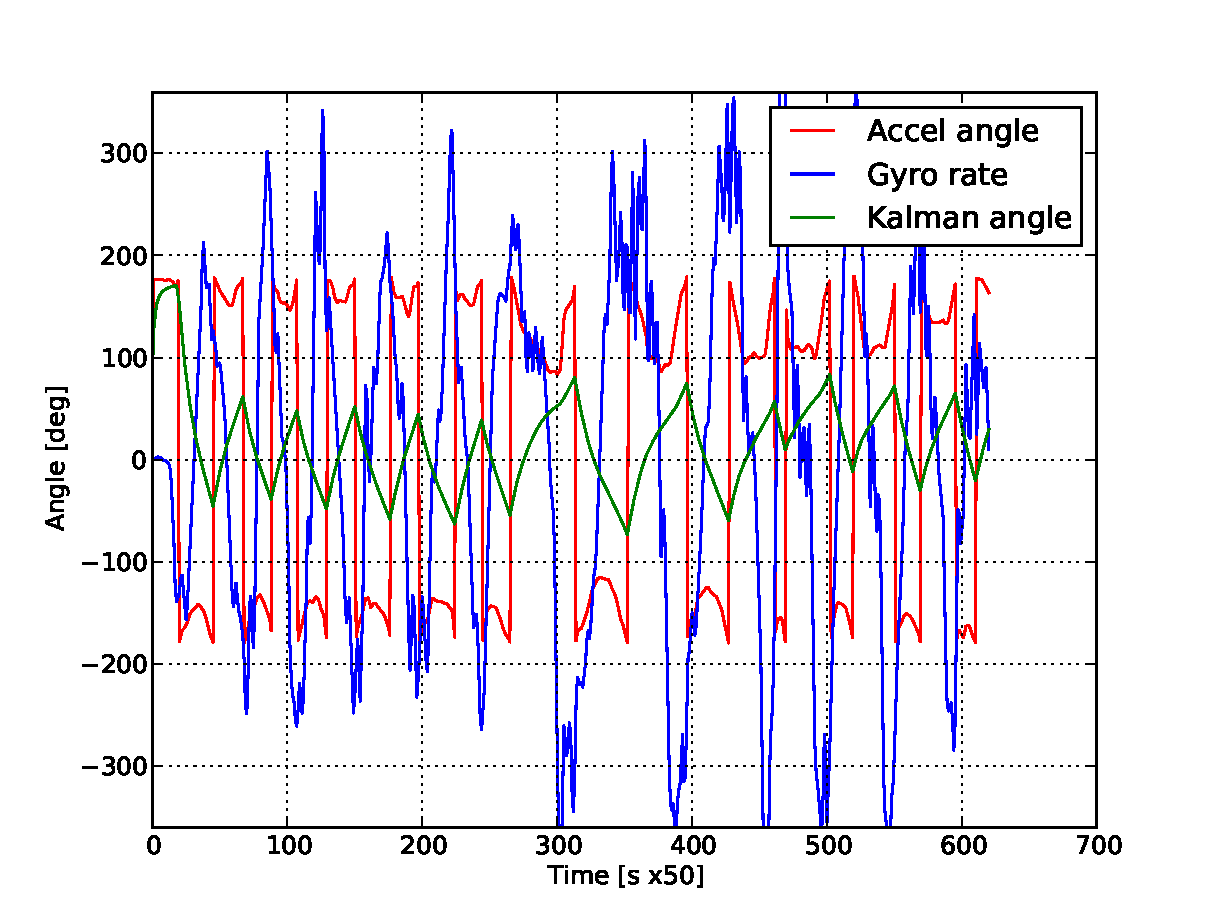
\includegraphics[scale=0.8]{fig/kalman_highfreq.pdf}
\caption{Kalman filter : High frequency input}
\label{fig:5_kalman_highfreq}
\end{figure}
Fig. \ref{fig:5_kalman_highfreq} has been plotted for a very high frequency movement of the IMU. As shown, the rates exceed 
$\pm320^o/s$ which is the maximum rate detected by the gyro. The final output of the kalman filter does match the hand movement
of about 90 degrees. However, at about the $300^{th}$ update, it completely misses a very fast 360 deg. rotation of the IMU. This
is reasonable because even the accelerometer and gyroscope do not seem to significantly register this movement.

\begin{figure}[!h]
\centering
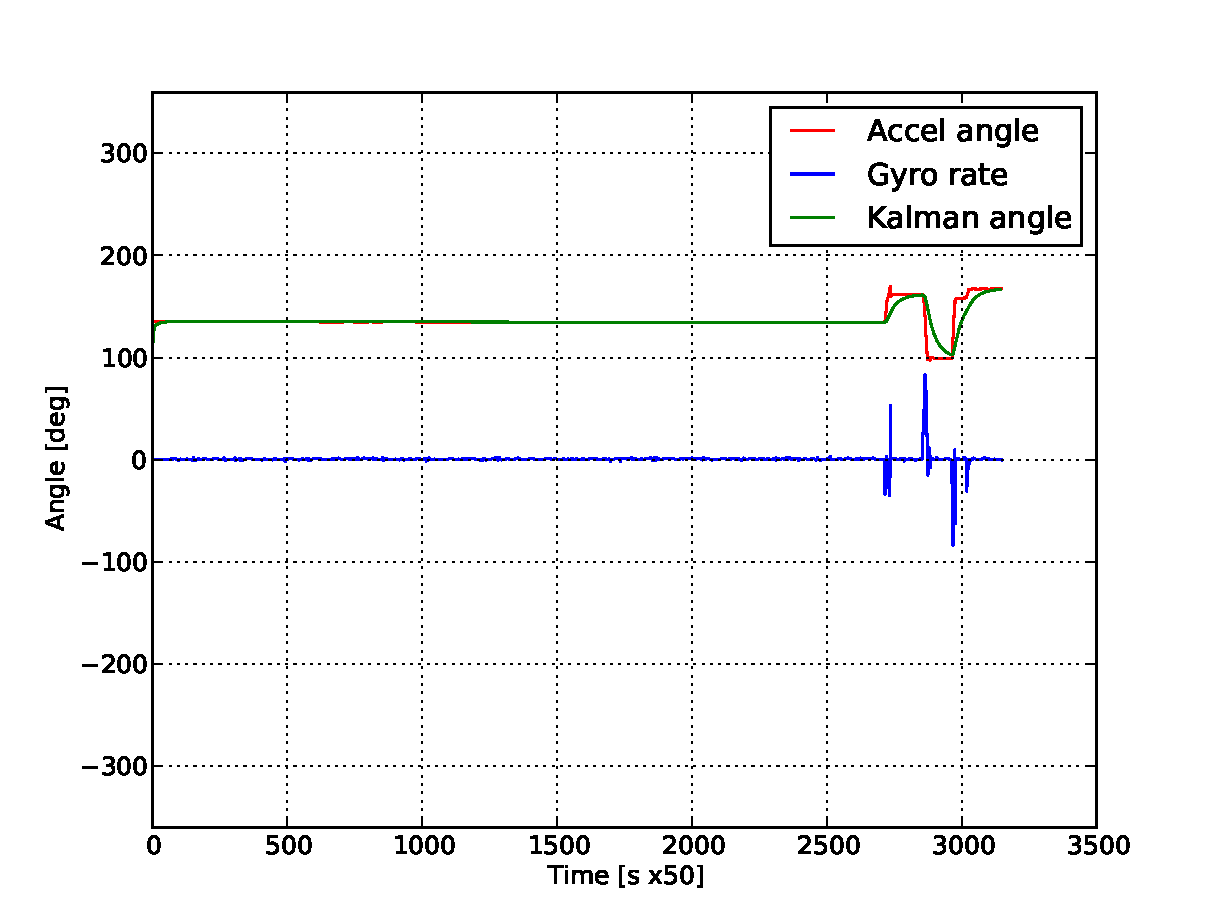
\includegraphics[scale=0.8]{fig/kalman_drift.pdf}
\caption{Kalman filter : Gyro drift}
\label{fig:5_kalman_gyrodrift}
\end{figure}
\newpage
Fig. \ref{fig:5_kalman_gyrodrift} shows readings plotted for 5 minutes at a 10 Hz update rate for the filter. It is seen that the
gyro rate has some noise. However, integrating this noise does not show a large error in the angle moved by the sensor. The
integral of the gyro rate is zero for all the time. The drift mentioned for gyroscopes is not to be seen even for periods as large as
12 minutes.

\section{Implementation}
We have to perform filtering on the onboard embedded system. It is essential that we finish off
the filtering part quickly so that the microcontroller can devote enough time to implementing
the control law. Polling data from the sensors also takes precious time. I set an update rate of 50 Hz
as the goal, this is also the maximum update rate of the gyroscope, so the filter cannot be run faster
than that. Two major parts of the implementation are as follows,

\subsection*{Inverse tan function}
The tilt of the accelerometer is obtained as follows,
\begin{equation}
\theta = tan^{-1} (\frac{a_y}{a_x})
\end{equation}
The C30 library provides an implementation of the $tan^{-1}$ function in floating point. However, these
operations take time on a 16-bit microcontroller. I thus implemented it using a table of stored values
and interpolating for values between them. The salient features of this are,
\begin{enumerate}
\item
\textit{tan} is an odd function, so we just need to include positive values in the table
\item
It is highly non-linear after 70 deg. So we will have a $tan^{-1}$ function only from -70 to +70 deg.
This gives a range of 140 deg. for the attitude which will be sufficient.
\item
Tangent function is linear enough till $15^{o}$, so we use this in our calculations. Divide the
interval $[$tan($15^{o}$), tan($70^{o}$)$]$ in 16 intervals. Store these \textit{tangents} and
the corresponding \textit{angles} in a table.
\item
Given a value, find out the interval within which it lies. Linearly interpolate \textit{tangent}
function within this interval.
\item
We identify a systematic``ish'' error of 0.06 deg in our implementation and hence add 0.06 deg.
while calculating the angle in the tabular implementation.
\item
This implementation requires just 48 bytes of memory and is computationally cheap as well.
\end{enumerate}
Fig. \ref{fig:5_atanD} shows the error between the $tan^{-1}$ function of the python math library
and $tan^{-1}$ function using the table above. We can implement this on the microcontroller using
fixed point arithmetic as shown in Sec. \ref{subsec:fp} to further reduce the computational time.
\begin{figure}[!h]
\centering
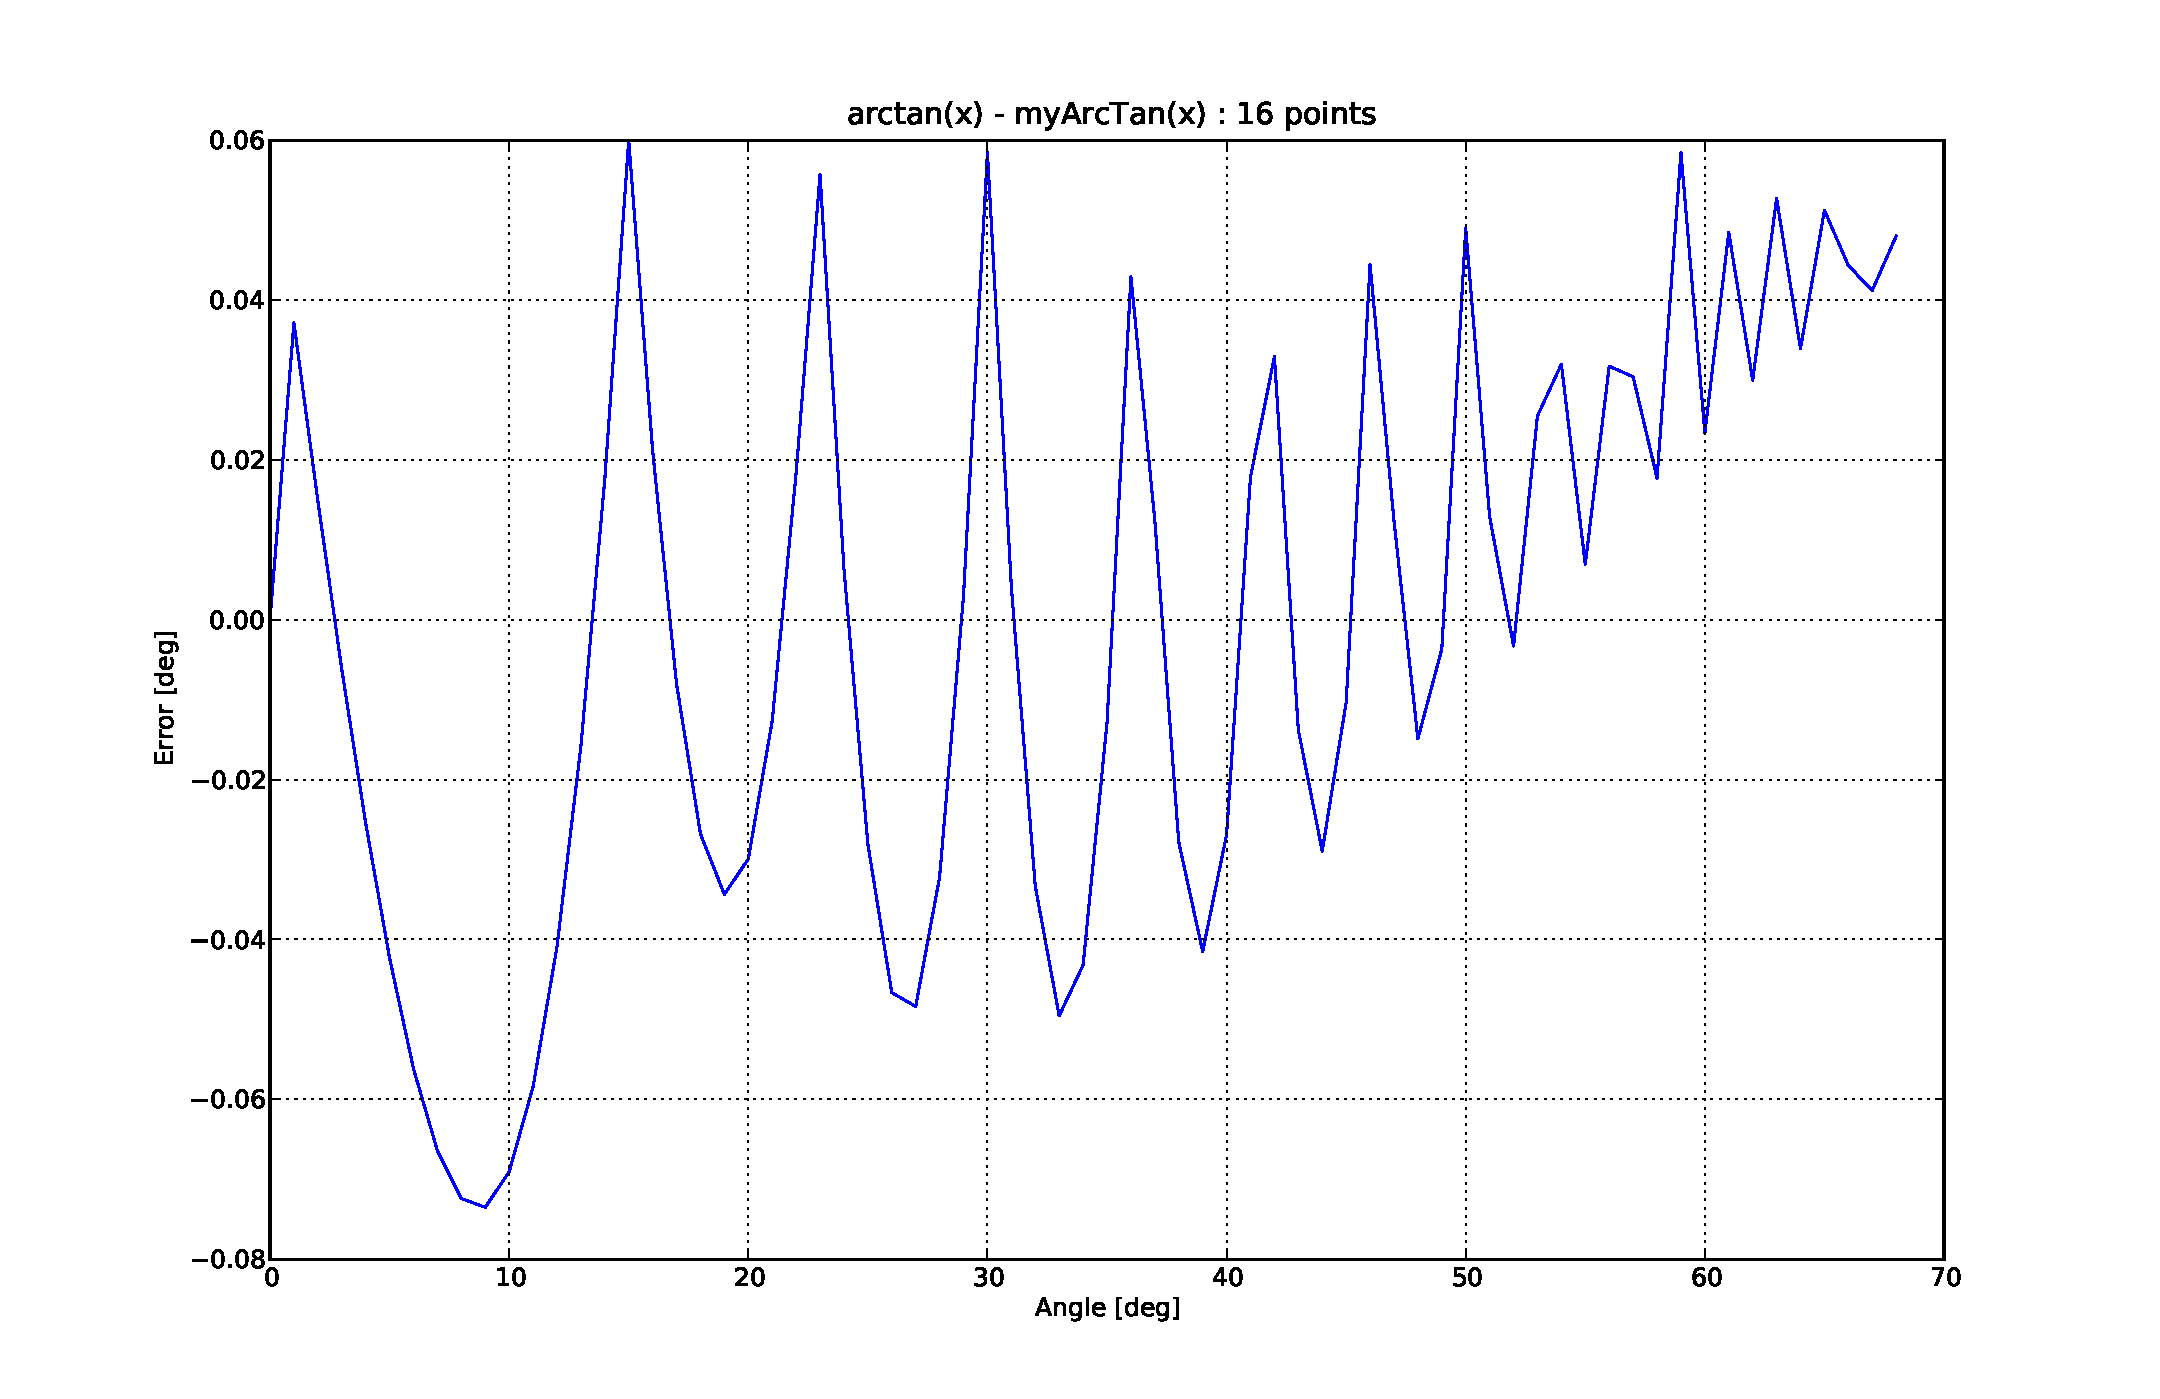
\includegraphics[scale=0.45]{fig/atanD.pdf}
\caption{$tan^{-1}$ function : Error between actual and the tabular implementation}
\label{fig:5_atanD}
\end{figure}

\subsection*{Fixed point arithmetic}
\label{subsec:fp}
There is one another way to reduce the computational overhead of the Kalman Filter. The accelerometer
provides the inclination values directly. It is known that the error in these values is $\pm0.5$ deg.
Implementing the tabular tangent function and the Kalman Filter in fixed point both is an option.
I however feel that the errors in the fixed point arithmetic will dominate over the inclinometer error
and hence it is not a bad idea to use the inclinometer directly. This will save some CPU cycles too.
Hence I implemented the Kalman Filter in fixed point arithmetic. The salient features are as follows,
\begin{enumerate}
\item
On a 16-bit microcontroller, we use 10.6 type signed fixed point numbers. The higher 10 bits are used
for the integer part of the number whereas the lower 6 bits are used for the mantissa. The
resolution of this scheme is thus $\frac{1}{2^{6}} = 0.015625$.
\item
Thus we have to scale every number by $2^{6} = 64$ before operating upon it. The Kalman
Filter constants are already hardcoded in the 10.6 form. The variables also operate and
get operated in this form itself.
\item
Multiply by 64 everytime two 10.6 fixed point numbers divide and divide by 64 everytime they get
multiplied to preserve the scaling.
\item
The integer part should be large enough to accomodate the rollover from the mantissa part after the
multiplication.
\item
Type-casting should be done properly while performing the arithmetic to prevent truncation by the
compiler.
\end{enumerate}

Figures \ref{fig:5_KF_fp_hf} and \ref{fig:5_KF_fp_lf} plot the tilt given by the accelerometers directly 
vs the fixed point implementation on the microcontroller vs the floating point implementation on a
computer. The floating point implementation on the computer
lags behind the microcontroller implementation slightly. This is probably because the covariance of the
accelerometer is a floating point number with a mantissa greater than 0.5 and is thus badly
rounded off in the fixed point implementation.
\newline
\begin{figure}[!h]
\centering
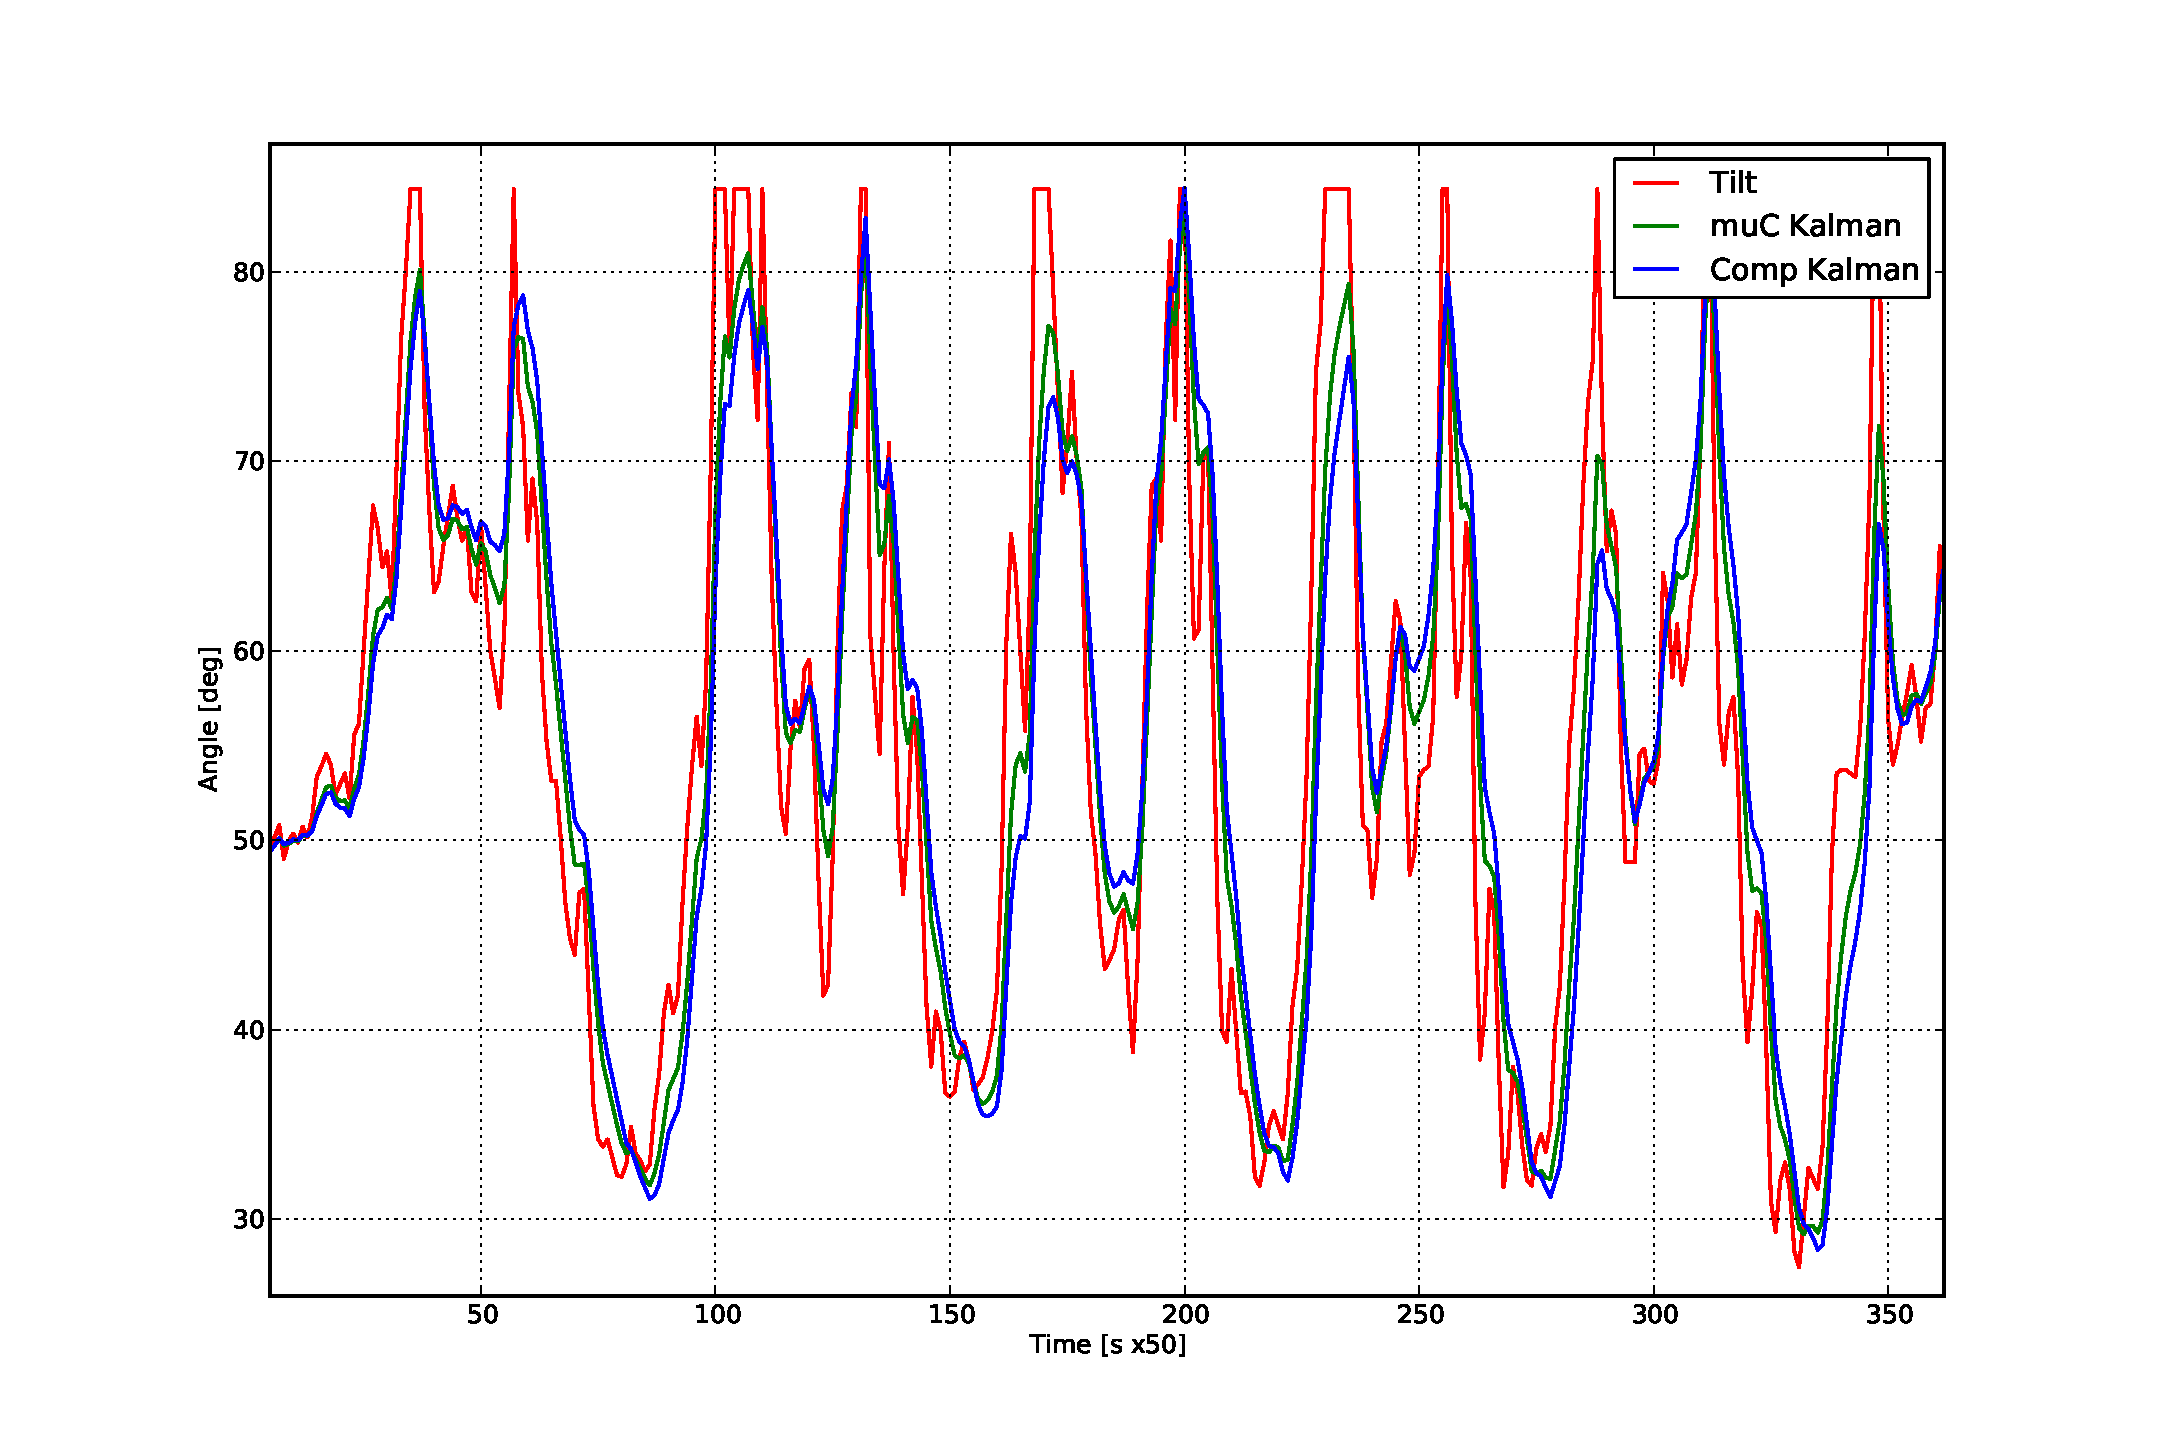
\includegraphics[scale=0.70, angle=270]{fig/kf_fp_hf.pdf}
\caption{Fixed point Kalman Filter : High freqency}
\label{fig:5_KF_fp_hf}
\end{figure}
\begin{figure}[!h]
\centering
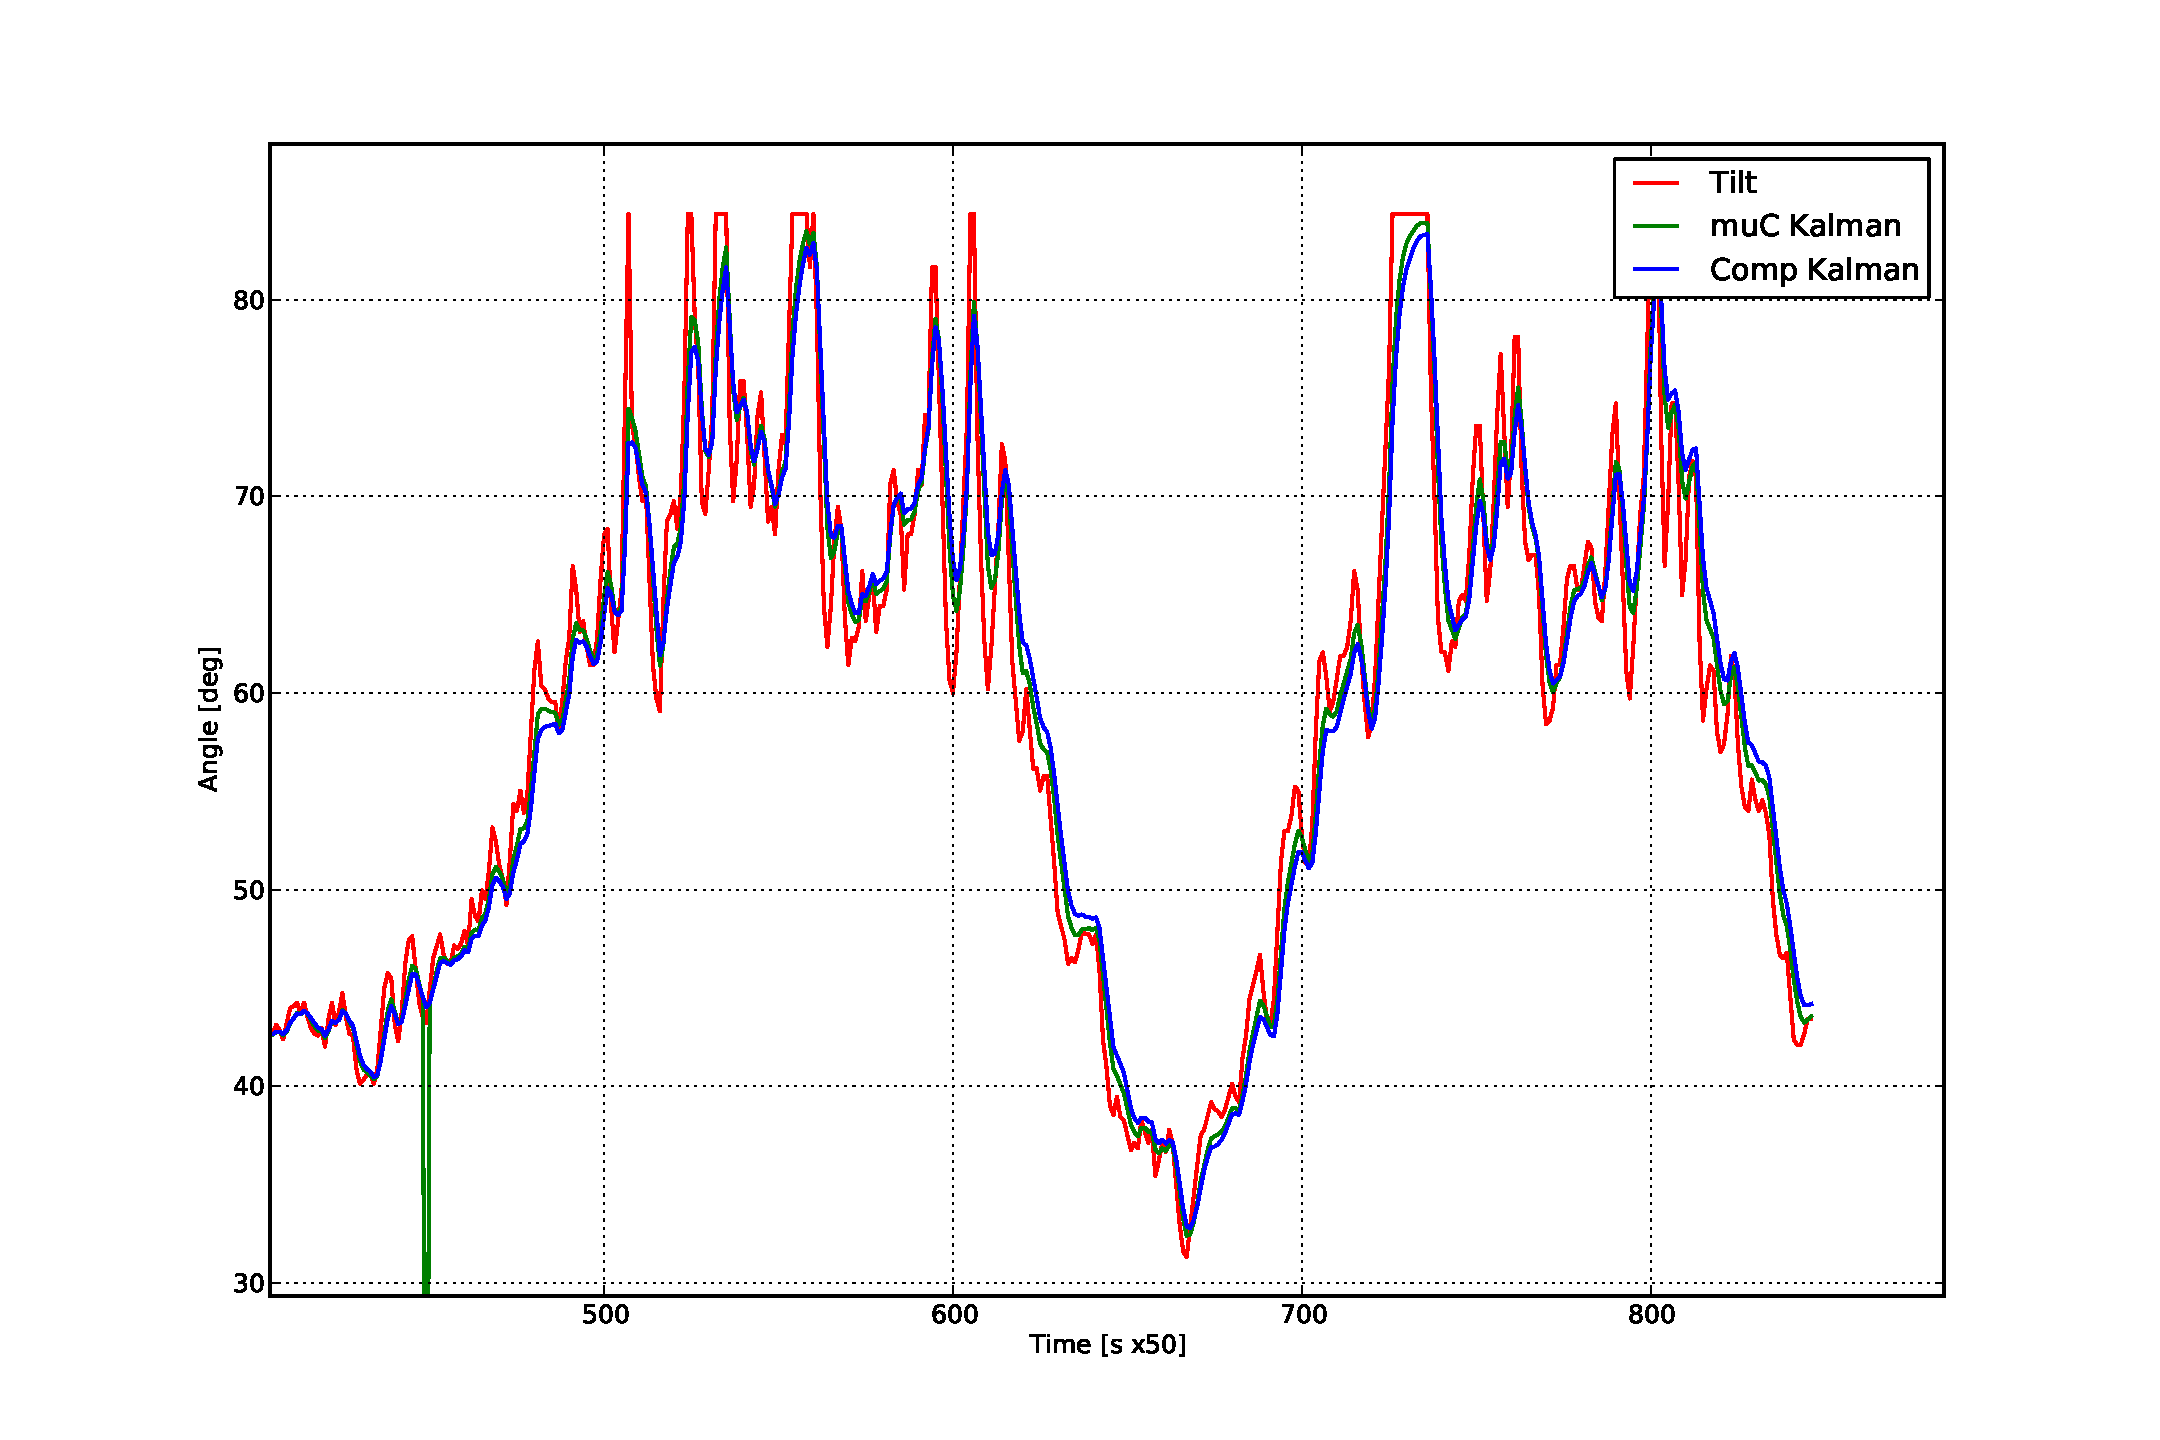
\includegraphics[scale=0.70, angle=270]{fig/kf_fp_lf.pdf}
\caption{Fixed point Kalman Filter : Low freqency}
\label{fig:5_KF_fp_lf}
\end{figure}

The source code for the fixed point implementation is given in the appendix.

















    \chapter{Conclusion}
\label{chap:conclude}

The project aimed to tackle four tasks viz.
\begin{enumerate}
  \item
  The essence of this phase was 
  to use a number of simple back-of-the-envelope style analyses to get an idea of the relative importance 
  of the enormous number of parameters associated with this system. Such analyses were instrumental in 
  getting an intuitive grasp of the complex dynamics without getting into mathematical complexities. It also helped a lot while performing design iterations to decide final dimensions.
  \item
  \begin{itemize}
   \item 
    This concentrated on the control aspect of the robot. I have modeled the 
    whole non-linear system for the hopping robot and simulated stable in-place hopping as well as a stable 
    hopping gait.
    \item
    I faced some limitations due to the nature of the computing environment (Mathematica) and hence I believe a lot of nicer things are possible like running a GA to get the good launch parameters automatically, finding an explicit Poincare Map and doing eigenvalue analysis and finally hopping over uneven terrain. There is a lot of scope for further work in terms of bifurcation analysis, path following, hopping with minimal expenditure of energy etc.
  \end{itemize}

  \item
  \begin{description}
   \item[\textsf{Mechanical}] 
    Another major task was to fabricate the robot. The robot is being fabricated and should be ready by this week . There was a lot of delay in getting the robot fabricated partly due to the hunt for a better design and partly due to the complexity of the mechanisms involved.
    \item[\textsf{Electronics}]
    The electronics has been designed and is ready. Essential tasks such as event detection, motor control and sensor filtering were duly concentrated upon to ensure enough computing power for the control law. Wireless debugging was extensively used to analyse codes.
  \end{description}
  \item
  Experimentation with the actual system was a crucial aspect of the project which couldn't be completed. 
  It will need another few weeks to get the robot up and running. I aim to convert the controller in 
  embedded form and demonstrate a running gait as further work.
\end{enumerate}

    {
\appendix
\chapter{Equations of motion}
\lstinputlisting{eqns.m}

\chapter{Kalman Filter Implementation}
\lstinputlisting{kalman_code.c}

    
}
    
    
    \newpage
    \addcontentsline{toc}{chapter}{References}
    \bibliography{ref}
    
    \newpage
\vspace*{0.75in}
\label{pg:ack}
\begin{center} {\bf \Huge Acknowledgment}\\[0.5in] \end{center}
{\normalsize I wish to express my sincere gratitude to Prof. Seth and Prof. Arya for supporting
and guiding me during the entire duration of this seminar.}\\


    \newpage
\vspace*{0.75in}
\label{pg:ack}
\begin{center} {\bf \huge Declaration of Integrity}\\[0.5in] \end{center}
{\normalsize I declare that this report represents my ideas in my own words and where others' ideas or words have 
been included, I have adequately cited and referenced the original sources. I also declare that I have adhered to 
all principles of academic honesty and integrity and have not misrepresented or fabricated or falsified any idea 
/ data / fact / source in my report. I understand that any violation of the above will be cause for disciplinary 
action as per the rules and regulations of the institute.}\\[1in]

\begin{center}
\raggedleft{\bf \large Pratik Chaudhari}\\[0.1in]
{\raggedleft \today\\[0.1in]}
\end{center}

\end{document}
